%**************************************************************************************************
%*  Nome: Nicolas P. Lane                                                                         *
%*  Data: 13/10/2015                                                                              *
%*  D�vidas ou contribui��es: lambdox@gmail.com                                                   *
%*  Modelo de monografia para TCC - UDESC de acordo com o manual de trabalhos acad�micos da UDESC *                                     *
%*  									                          *
%*  Licen�a GPL:              						                          *
%*  Permission to use, copy, modify, and distribute this protocol and its                         *
%*  documentation for any purpose, without fee, and without written                               *
%*  agreement is hereby granted, provided that the above copyright notice,                        *
%*  and the author appear in all copies of this protocol.                                         *
%**************************************************************************************************

\NeedsTeXFormat{LaTeX2e}
%-----------------------------------------------------------
\documentclass[a4paper,12pt]{monografia}
\usepackage{amsmath, amsthm, amsfonts, amssymb}
\usepackage[english, brazilian]{babel}
\usepackage[titletoc]{appendix}
\usepackage[latin1]{inputenc}
\usepackage[mathcal]{eucal}
\usepackage[alf]{abntcite}
\usepackage{subfigure}
\usepackage{isoaccent}
\usepackage{textcase}
\usepackage{multirow}
\usepackage{latexsym}
\usepackage{graphicx}
\usepackage{listings}
\usepackage{acronym}
\usepackage{bm}
\lstset{basicstyle=\tiny, language=C++}
\makeindex			
%-----------------------------------------------------------Come�a documento
\begin{document}
%----------------- T�tulo e Dados do Autor -----------------
\titulo{Seu t\'itulo}
\autor{Seu nome}
\nome{Seu nome do meio}
\ultimonome{Seu \'ultimo nome}

%---------- Informe o Curso e Grau -----
\bacharelado \curso{Ci\^encia da Computa\c{c}\~ao} \mes{Junho} \ano{2015} 
\data{\today} % data da aprova��o
\cidade{Joinville}

%----------Informa��es sobre a Institu��o -----------------
\instituicao{Universidade do Estado de Santa Catarina}
\sigla{UDESC} \unidadeacademica{Centro de Ci\^encias Tecnol\'ogicas}

%------Nomes do Orientador, 1o. Examinador e 2o. Examinador-
\orientador{Nome completo do orientador 1}
\examinadorum{Nome completo do orientador 2}
\examinadordois{Nome completo do orientador 3}
%\examinadorquatro{Nome do Examinador 4}

%--------- T�tulos do Orientador 1o. e 2o. Examinadores ----
\ttorientador{T\'itulo do orientador 1}
\ttexaminadorum{T\'itulo do orientador 2}
\ttexaminadordois{T\'itulo do orientador 3}
%\ttexaminadorquatro{T�tulo do Examinador 4}

\maketitle
%---------------------- AGRADECIMENTO --------------
\agradecimento{Agradecimentos}

  AAAAAAAAAAAAAAAAAAAAAAAAAAAAAAAAAAAAAAAAAAAAAA AAAAAAAAAAAAAAAAAAAAAAAAAAAAAAAAAAA AAAAAAAAAAAAAAAAAAAAAAAAAAAAAAAAAAAAAAAAAAAAAA 
AAAAAAAAAAAAAAAAAAAAAAAAAAAAAAAAAAA AAAAAAAAAAAAAAAAAAAAAAAAAAAAAAAAAAAAAAAAAAAAAA AAAAAAAAAAAAAAAAAAAAAAAAAAAAAAAAAAA 
AAAAAAAAAAAAAAAAAAAAAAAAAAAAAAAAAAAAAAAAAAAAAA AAAAAAAAAAAAAAAAAAAAAAAAAAAAAAAAAAAAAAAAAAAAAA AAAAAAAAAAAAAAAAAAAAAAAAAAAAAAAAAAA 
AAAAAAAAAAAAAAAAAAAAAAAAAAAAAAAAAAA

\newpage
%---------------------- EP�GRAFE --------------
\begin{epigrafe}

  Disce Docendo Adhuc

\end{epigrafe}
%--------Digite aqui o seu resumo em Portugu�s--------------
\resumo{Resumo}
A crescente popularização de jogos \acf{mmorpg} demanda por novas abordagens tecnológicas, a fim de suprir as necessidades dos usuários com menor custo de recursos computacionais.
%
Projetar essas arquiteturas, do ponto de vista da rede, é algo pertinente e impactante para o sucesso desses jogos.
%
O objetivo deste trabalho é propor uma análise voltada a identificar os recursos computacionais consumidos pelas arquiteturas identificadas.
%
Esse objetivo será atingido após realizar uma pesquisa referenciada, seguida de uma análise das principais arquiteturas e, preferencialmente, a execução de simulações de clientes usando as arquiteturas implantadas em uma nuvem computacional para auxiliar na identificação de gargalos de recursos. 
%
Os resultados obtidos auxiliarão provedores de serviços \ac{mmorpg} a reduzir gastos de manutenção e melhorar a qualidade de tais serviços.
%chamada de arquivo resumo.tex

\noindent Palavras-chaves: Comunica��o Alternativa, Paralisia Cerebral, defici�ncia na fala, software livre
%-----------Digite aqui o seu resumo em Ingl�s--------------
\resumo{Abstract}
The increasing popularization of mass games demands new technological approaches in order to meet the needs of users with lower cost of computational resources.
%
Designing these architectures, from the network point of view, is relevant and impacting to the success of these games.
%
The objective of this work is to propose an analysis aimed at identifying approaches to optimize the computational resources consumed by the identified architectures.
%
This objective will be achieved after conducting a referenced search, followed by an analysis of the main architectures and, respectively, the execution of simulations using a computational cloud to assist in the identification of resource bottlenecks.
%
The results obtained will help \ac{mmorpg} service providers to reduce maintenance costs and improve the quality of such services.     %chamada de arquivo abstract.tex

\noindent Keywords: Alternative Comunication, Cerebral Palsy, speech deficiency, open source
%-----------------------------------------------------------

\listoffigures       %gera p�gina com lista de figuras a partir de todas as entradas feitas no documento

% lista de abrevia��es
\listoftables        %gera p�gina com lista de tabelas a partir de todas as entradas feitas no documento
\listofabbreviations{Lista de Abreviaturas}
\begin{acronym}[]
	\acro{amqp}[AMQP]{{\it Advanced Message Queuing Protocol}}
	\acro{api}[API]{{\it Application Programming Interface}}
    \acro{aws}[AWS]{{\it Amazon Web Services}}
	\acro{cli}[CLI]{{\it Command Line Interface}}
	\acro{ddos}[DDoS]{{\it Distributed Denial of Service}}
	\acro{iaas}[IaaS]{{\it Infrastructure as a Service}}
    \acro{ids}[IDS]{{\it Intrusion Detection System}}
	\acro{kvm}[KVM]{{\it Kernel-based Virtual Machine}}
    \acro{ldap}[LDAP]{{\it Lightweight Directory Access Protocol}}
	\acro{nist}[NIST]{{\it National Institute of Standards and Technology}}
	\acro{paas}[PaaS]{{\it Platform as a Service}}
    \acro{rpc}[RPC]{{\it Remote Procedure Call}}
	\acro{saas}[SaaS]{{\it Software as a Service}}
	\acro{snmp}[SNMP]{{\it Simple Network Management Protocol}}
	\acro{qos}[QoS]{{\it Quality of Service}}
	\acro{sdn}[SDN]{{\it Software Defined Network}}
	\acro{vlan}[VLAN]{{\it Virtual Local Area Network}}
	\acro{vm}[VM]{{\it Virtual Machine}}
	\acro{vpn}[VPN]{{\it Virtual Private Network}}

	\acro{POV}[POF]{{\it Point of View}}

	\acro{FPS}[FPS]{{\it First-person shooter}}
	\acro{TPS}[TPS]{{\it Third-person shooter}}
	\acro{RTS}[RTS]{{\it Real-time strategy}}
	\acro{MMO}[MMO]{{\it Massively multiplayer online}}
	\acro{RPG}[RPG]{{\it Role-playing game}}
	\acro{MMORPG}[MMORPG]{{\it Massively multiplayer online role-playing game}}
	\acro{MOBA}[MOBA]{{\it Multiplayer online battle arena}}
	\acro{MMOFPS}[MMOFPS]{{\it Massively multiplayer online first-person shooter}}

	\acrodefplural{vpn}[VPNs]{{\it Virtual Private Networks}}
	\acrodefplural{vlan}[VLANs]{{\it Virtual Local Area Networks}}
	\acrodefplural{vm}[VMs]{{\it Virtual Machines}}
\end{acronym}

% Defining: \acro{acronym}[short name]{full name}
% Usaging:
% \ac{acronym}     -- writes the full name followed by the acronym in brackets; later calls will write only the acronym
% \acf{acronym}     -- writes the full name followed by the acronym in brackets
% \acs{acronym}     -- writes the short name only
% \acl{acronym}     -- writes the full name only
% Use p at the end of previous commands for plural form (e.g., \acp for the plural form of \ac)
% \acresetall        -- reset usage of all acronyms (i.e., \ac will print full name again)
% \acused                -- mark the acronym as used
    %chamada de arquivo acronimos.tex

%----Sum�rio, lista de figura e de tabela ------------
\tableofcontents      %gera p�gina com sum�rio a partir de todas as entradas feitas no documento

%--------------In�cio do Conte�do---------------------------
\pagestyle{ruledheader} %estilo abnt2
\chapter{Introdu��o}
\label{cap:introducao1}


A acessibilidade � a possibilidade de qualquer pessoa, independentemente de suas capacidades f�sico-motoras e perceptivas, culturais e sociais, usufruir os benef�cios de uma vida. Al�m disso, a acessibilidade tem como objetivo possibilitar o acesso de pessoas com defici�ncia permanente ou tempor�ria (e.g., f�sicas, auditivas, etc.) na sociedade afim de que todas possam participar ativamente.

Para que o objetivo da acessibilidade seja cumprido, � necess�rio o estudo e cria��o de alternativas, para que estas pessoas possam contornar ou compensar algum tipo de defici�ncia que as impe�a a sua inser��o. Essa demanda motivou o surgimento da \acf{TA}, uma parte da tecnologia que deve ser entendida como um aux�lio que promove a amplia��o de uma habilidade funcional deficit�ria ou possibilitar a realiza��o da fun��o desejada e que se encontra impedida. Contudo, ainda s�o encontradas muitas dificuldades, principalmente pelo tema ser consideravelmente novo, a quantidade de trabalhos cient�ficos relacionado ao tema ainda � pouco expressivo.

Nas diferentes classifica��es da \ac{TA}, existe a \acf{CAA} que pode ser definida como uma alternativa a comunica��o escrita e oral. A \ac{CAA} inicialmente era composta apenas de sistemas sem tecnologia, como libras, cart�es e livros. Por�m, com o avan�o da tecnologia nas �ltimas d�cadas, sistemas anal�gicos e sistemas com recursos computacionais foram aumentando o escopo e as alternativas de \ac{CAA}.

Com uma quantidade expressiva de pessoas com algum tipo de paralisia no Brasil e no mundo, meios alternativos de inclus�o s�o necess�rios, principalmente meios alternativos dispon�veis a popula��o com baixa renda. Um dos objetivos espec�ficos do trabalho � analisar e diferenciar solu��es de \ac{CAA} que possibilitam a estimula��o cognitiva de pessoas com \acf{PC} em especial as pessoas que possuem habilidades locomotoras limitadas em conjunto com dificuldades na fala. Ap�s esta an�lise, verificar se � necess�ria a implementa��o de uma solu��o alternativa a essas pessoas. Contudo, esta s� pode ser atingida atrav�s de estudos sobre \ac{PC} e os requisitos que estas solu��es demandam. O principal objetivo do trabalho resume-se em implementar um software para computador alternativo de \ac{CAA} de licen�a GPL, para que pessoas com \ac{PC} possam ter seus c�rebros estimulados cognitivamente. 

A organiza��o deste trabalho est� dividida em quatro cap�tulos, ``Conceitos B�sicos'', ''Defini��o do Problema'', ``Proposta'' e ``Considera��es''. No primeiro cap�tulo s�o apresentados a quantidade de pessoas com defici�ncia no Brasil e no mundo, defini��es e legisla��o sobre \ac{TA} e \ac{TA} dentro da inform�tica, tamb�m � abordado as pessoas que possuem \ac{PC} e seus diferentes casos. Al�m disso, tamb�m estuda-se as principais iniciativas de \ac{TA} pelo mundo e seus termos e classifica��es. Ao final do cap�tulo � apresentado as defini��es de \ac{CAA} os seus recursos e estrat�gias e quais os termos e classifica��o que ser�o utilizados no trabalho.

No segundo cap�tulo, � definido o problema e os usu�rios finais da solu��o. O trabalho nesta parte levanta problemas com a prancha de comunica��o, que � a solu��o atual dos terapeutas, e ap�s isso identifica os requisitos necess�rios para o desenvolvimento da solu��o atrav�s de entrevista com uma psic�loga especialista em reabilita��o de pessoas com \ac{PC}. Ao final s�o identificados trabalhos correlatos e apresentado uma compara��o com base nos requisitos levantados.

No terceiro cap�tulo, � elaborado uma especifica��o da proposta, determinando os m�todos que ser�o utilizados para cumprir os requisitos levantados. Atrav�s de diagramas das tarefas, diagramas de classe e de estados da solu��o o trabalho indica quais ser�o as intera��es do usu�rio com a solu��o. S�o mencionados tamb�m os limitadores e e plano de teste que tem como objetivo fazer com que a solu��o evolua no decorrer do trabalho. 

\chapter{Conceitos}
\label{cap:introducao}
\acresetall
Ao longo da hist�ria em rela��o �s pessoas com defici�ncia, � poss�vel encontrar uma variedade de termos que foram se modificando ao longo dos anos: ``Inv�lidos'', ``incapacitados'', ``defeituosos'', ``excepcionais'' s�o alguns exemplos de termos atribu�dos �s pessoas com defici�ncia em diferentes �pocas. Os termos s�o considerados corretos em fun��o de valores e conceitos vigentes em cada sociedade e em cada �poca, portanto, os termos supracitados foram aceitos, usados e, em dados momentos da hist�ria, substitu�dos. No estudo da evolu��o do conceito da defici�ncia encontra-se que, em 1980, a Organiza��o Mundial de Sa�de prop�s a utiliza��o da CIDID - Classifica��o das Defici�ncias, Incapacidades e Desvantagens\cite{cidid} ({\it Handicaps})\footnote{Termo em ingl�s traduzido como defici�ncia} com intuito de organizar uma linguagem universal a respeito das defici�ncias. A implementa��o de uma nova terminologia, ``pessoas deficientes'', passou a atribuir o valor de pessoa a aqueles que at� ent�o eram desconsiderados como tais pela sociedade. Ressalta-se que a revis�o dessas nominatas teve a preocupa��o de centrar-se na pessoa e n�o na defici�ncia \cite{fiquene,chagas}.

Segundo a \citeonline{onu}, existem no mundo 1 bilh�o de pessoas que possuem algum tipo de defici�ncia. Segundo o Censo de 2010 \cite{censo} a ocorr�ncia de pessoas com defici�ncia na popula��o brasileira � de 23,9\% da popula��o. A tabela \ref{tabela_pop} apresenta a distribui��o dos tipos de defici�ncia no Brasil.


\begin{table}[bth!]
\centering
\scriptsize
\caption{Distribui��o dos tipos de defici�ncia no Brasil.}\vspace{.2cm}

	
    \begin{tabular}{ | l | l |}
		
    \hline
    Condi��o & Por��o da Popula��o\\ \hline \hline
    Defici�ncia Visual & 18,6\%\\ \hline
		Defici�ncia Motora & 7\%\\ \hline
		Defici�ncia Auditiva & 5,1\%\\ \hline
		Defici�ncia Mental ou Intelectual & 1,4\%\\ \hline
		
    \end{tabular}
    \label{tabela_pop}
		\vspace{0.1cm}\\Fonte: o pr�prio autor com base no Censo de 2010\cite{censo}.

\end{table}



A tabela \ref{tabela_pop} mostra que na popula��o brasileira, 18,6\% da popula��o possuem defici�ncia visual sendo a defici�ncia mais recorrente entre os brasileiros. A defici�ncia motora, a segunda com maior recorr�ncia, � apresentada em 7\% da popula��o, seguida da defici�ncia auditiva com 5,1\%, e das pessoas com defici�ncia mental que apresentam 1,4\%. Na tabela \ref{tabela_pop} a soma das porcentagens n�o � igual a 23,9\% pois algumas pessoas possuem mais de uma defici�ncia citada. Outro fator importante � que 65\% das pessoas que possuem algum tipo de defici�ncia recebem menos de dois sal�rios m�nimos no Brasil\cite{censo}, sendo que 10\% dessas pessoas tem renda de menos da metade de um sal�rio m�nimo. 

As pessoas que possuem algum tipo de defici�ncia sofrem dificuldades ao acesso das necessidades b�sicas conquistadas pelo ser humano, segundo o Programa de A��o Mundial para Pessoas Deficientes da ONU\cite[p.~11]{onu},

\begin{quotation}''[...] a experi�ncia tem demonstrado que, em grande medida, � o meio que determina o efeito de uma
incapacidade sobre a vida cotidiana da pessoa. A pessoa v�-se relegada � invalidez quando
lhe s�o negadas as oportunidades de que disp�e, em geral, a comunidade, e que s�o
necess�rias aos aspectos fundamentais da vida, inclusive a vida familiar, a educa��o, o
trabalho, a habita��o, a seguran�a econ�mica e pessoal, a participa��o em grupos sociais e
pol�ticos, as atividades religiosas, os relacionamentos afetivos e sexuais, o acesso �s
instala��es p�blicas, a liberdade de movimenta��o e o estilo geral da vida di�ria [...]''.
\end{quotation} 

Neste trabalho � dada �nfase a pessoas com defici�ncia motoras, mais especificamente as pessoas que possuem \ac{PC}.  A Encefalopatia Cr�nica da Inf�ncia (E.C.I.), tamb�m conhecida como \ac{PC}, � uma doen�a cr�nica de car�ter n�o evolutivo, que em 90\% das vezes possuem defici�ncia f�sica. O curso natural das les�es � de longa dura��o, necessitando a crian�a de tratamento prolongado. Tem efeitos n�o apenas sobre o crescimento e o desenvolvimento f�sico, mas tamb�m sobre a destreza, a personalidade, a capacidade cognitiva, as atitudes pessoais e sociais do paciente, as emo��es e as intera��es da fam�lia\cite{leite,sa}. Como a \ac{PC} possui diferentes tipos de manifesta��es e graus da doen�a, para maior compreendimento das necessidades de pessoas com \ac{PC}, � necess�rio conhecer os diferentes quadros cl�nicos da doen�a. 


\section{Quadro Cl�nico: \acf{PC}}

Existem v�rios quadros cl�nicos de pessoas, que possuem \ac{PC}, e podem ser beneficiadas por algum recurso que facilite a sua comunica��o com outras pessoas. Neste sentido alguns quadros se encaixam melhor ou pior a determinadas facilidades de comunica��o. As poss�veis causas da \ac{PC} (e.g., causas pr�-natais, perinatais e p�s-natais) n�o ser�o tratadas, pois n�o pertencem ao escopo deste trabalho.
Na observa��o cl�nica da \ac{PC}, deve-se levar em considera��o a extens�o do dist�rbio motor, sua intensidade e, principalmente, a caracteriza��o semiol�gica\footnote{Caracteriza��o semiol�gica, refere-se a caracteriza��o dos sinais e sintomas da doen�a.} desse dist�rbio\cite{leite}. Assim, a paralisia cerebral apresenta v�rias formas cl�nicas que s�o apresentadas na tabela \ref{tabela}.

\begin{table}[bth!]
\centering
\scriptsize
\caption{Tabela com os diferentes casos de \ac{PC}.}\vspace{.2cm}

	
    \begin{tabular}{ | l |  p{7cm} | p{5cm} |}
		
    \hline
    Quadro & Descri��o das Limita��es  & Aplic�vel recurso de comunica��o\\ \hline \hline
    Hemiplegia &   Sinais de libera��o tais como espasticidade , hiper reflexia e sinal de Babinski & Aplic�vel em alguns graus \\ \hline
    Hemiplegia bilateral & Tetra ou quadriplagia, dependendo do grau defici�ncia mental e epilepsia & Aplic�vel a pacientes com menor grau de les�o \\ \hline
    Diplegia & Com\-pro\-me\-ti\-men\-to dos membros inferiores, co\-mu\-men\-te evidenciando uma acentuada hipertonia dos adutores & Aplic�vel em alguns graus \\
    \hline
		Discinesia & Movimentos involunt�rios, ondulantes e repetidos com grande amplitude de movimento e incoordena��o motora &  Aplic�vel em alguns graus \\
    \hline
		Ataxia &  Perda de coordena��o dos movimentos musculares volunt�rios & Aplic�vel em alguns graus \\
    \hline
		Formas mistas & Combina��o dos quadros anteriores & Casos avaliados individualmente \\
    \hline
		
    \end{tabular}
    \label{tabela}
		Fonte: o pr�prio autor com base \citeonline{leite}.

\end{table}


A Tabela {\ref{tabela}} apresenta os diferentes quadros de \ac{PC}. Atrav�s dela pode-se perceber que independente do quadro, o grau da les�o de cada paciente com \ac{PC} tem que ser avaliado individualmente, para que se identifique quais s�o as necessidades de acessibilidade de cada um deles.  Para maiores informa��es sobre cada quadro cl�nico, ver Ap�ndice {\ref{apendice1}.



%No Brasil existem diversos movimentos sociais, dos mais variados �mbitos,voltados a ajudar as pessoas com defici�ncias. Tratando-se das pessoas com \ac{PC} os movimentos sociais tamb�m s�o decisivos. No entanto, os recursos normas e leis de acessibilidade ainda que claros, s�o parcialmente esquecidos pela sociedade e pela falta de investimento e pesquisa na �rea.As dificuldades encontradas s�o grandes, pois s�o poucas as literaturas especializadas e faltam equipamentos acess�veis a esse grupo da popula��o.

\section{Acessibilidade}

A acessibilidade � a possibilidade de qualquer pessoa, independentemente de suas capacidades f�sico-motoras e perceptivas, culturais e sociais, usufruir os benef�cios de uma vida em sociedade. � a possibilidade de participar de todas as atividades, at� as que incluem o uso de produtos, servi�os e informa��o, com o m�nimo de restri��es poss�vel \apud{nicholl,nbr}{unirio}.

As discuss�es sobre acessibilidade v�m crescendo no Brasil e no mundo \cite{donatangelo}.
O termo acessibilidade � muito amplo e, de certa forma, complexo de ser definido,
pois n�o pode ser entendido apenas como a facilidade de se ter acesso. Contudo, pode-se
caracterizar, de um modo geral, acessibilidade como sendo um processo din�mico que visa �
elimina��o de barreiras para que se tenha acesso.

A acessibilidade tamb�m � conhecida por ser a possibilidade e condi��o de alcance para a utiliza��o, com autonomia, simplicidade, efici�ncia e seguran�a, dos espa�os, mobili�rios, das edifica��es, dos equipamentos urbanos, dos transportes, dos sistemas e meios
de comunica��o e da inform�tica, por qualquer pessoa, sejam elas crian�as, adultos, idosos, contendo, ou n�o, necessidades especiais devido alguma defici�ncia ou mobilidade reduzida \apud{torres}{donatangelo}. No Brasil h� legisla��o que trata de quest�es de acessibilidade aos portadores de necessidades especiais. A legisla��o mais relevante no contexto deste trabalho s�o:
\begin{itemize}
\item Portaria n� 1.679, de dezembro de 1999, disp�e sobre requisitos de acessibilidade de 
pessoas portadoras de defici�ncias, para instruir os processos de autoriza��o e de 
reconhecimento de cursos, e de credenciamento de institui��es. 
 \cite{mec};
\item Lei n� 10.098, de dezembro de 2000, que, entre outras coisas, estabelece
normas gerais e crit�rios b�sicos para que seja promovida a acessibilidade
para pessoas com defici�ncia \cite{brasil}; e
\item Decreto n� 3.294, de dezembro de 1999, que instituiu o programa
Sociedade da Informa��o, na qual um dos objetivos � a universaliza��o do
acesso � Internet \cite{brasil1}.
\end{itemize}


Com a legisla��o presente, principalmente pelo decreto n� 3.294 a Acessibilidade ultrapassa as barreiras do espa�o f�sico e chega ao espa�o digital. No espa�o digital s�o encontradas muitas dificuldades, entre elas podem ser citadas a falta de
recursos tecnol�gicos, a falta de acesso aos recursos existentes e a falta de preocupa��o em
disponibilizar a informa��o de forma clara\apud{torres1}{donatangelo}. A utiliza��o de dispositivos eletr�nicos (e.g., computadores, {\it tablets} e { \it smart\-pho\-nes}) e o acesso � Internet permitem aos cidad�os acessarem um conjunto consider�vel de fontes de informa��o, estabelecerem contatos e trocarem
informa��es, exercerem uma atividade social e encontrarem formas alternativas de lazer e de
divertimento \apud{abra}{donatangelo}. Para que ocorra o mesmo com pessoas portadoras de algum tipo de defici�ncia, a acessibilidade na inform�tica � necess�ria.



\subsection{Acessibilidade na Inform�tica}

Para que a acessibilidade na inform�tica ocorra, � necess�rio levar em considera��o a redund�ncia, a simplicidade e a facilidade para compreens�o da informa��o\cite{torres}. A web desempenha um papel fundamental no avan�o que a Internet representa no cotidiano das pessoas com defici�ncia, facilitando a vida deles; ela permite que eles criem novas formas de relacionamento, encontrem oportunidades de trabalho e formas alternativas de divers�o \cite{torres}.

Atualmente a maioria dos web sites t�m barreiras de acessibilidade que dificultam ou mesmo tornam imposs�vel para estas pessoas acessarem sites. Contudo, se os web sites e softwares forem projetados levando em considera��o a acessibilidade, estas pessoas poder�o usar os sites efetivamente\cite{wc}.

Em maio de 1999 os membros do \ac{W3C} elaboraram o ``Estatuto de Recomenda��o do \ac{W3C}'' (WCAG 1.0), esse documento constitui a primeira vers�o das Diretrizes para a Acessibilidade ao Conte�do da web. Al�m disso, no Brasil o governo disponibiliza em seu site oficial o \ac{eMAG} \cite{emag} que consiste em um conjunto de recomenda��es a ser considerado para que o processo de acessibilidade dos sites e portais do governo brasileiro seja conduzido de forma padronizada e de f�cil implementa��o. O \ac{eMAG} � coerente com as necessidades brasileiras e em conformidade com os padr�es internacionais. Foi formulado para orientar profissionais que tenham contato com publica��o de informa��es ou servi�os na Internet a desenvolver, alterar e ou adequar p�ginas, web sites e portais, tornando-os acess�veis ao maior n�mero de pessoas poss�vel. 

Apesar de importante, a acessibilidade digital e na web n�o � t�o simples \cite{harrison}. Por exemplo, pessoas com defici�ncia possuem limita��es sensoriais e motoras que devem ser compensadas de alguma forma, a fim de viabilizar o acesso dessas pessoas aos recursos computacionais e, para isso, as organiza��es necessitam adaptar seu hardware e seus sistemas, a fim de fazer com que um computador possa ser usado por pessoas com defici�ncia \cite{harrison}. 

A acessibilidade digital, faz com que pessoas, que possuem algum tipo de defici�ncia, tenham acesso ao conte�do disponibilizado na web. Por�m, ainda existem barreiras em web sites, softwares, e algumas defici�ncias fazem com que as pessoas tenham limita��es sensoriais e/ou motoras. Sendo assim, � necess�rio um meio de compensar estas dificuldades para garantir o acesso a essas informa��es.


\section{Tecnologia Assistiva}
\label{Tecnologia Assistiva}

O termo {\it Assistive Technology}, traduzido no Brasil como \ac{TA} ou tamb�m conhecido como Ajudas T�cnicas, foi adotado no Brasil ap�s ser criado em 1988, como importante elemento jur�dico dentro da legisla��o norte-americana conhecida como {\it Public Law 100-407} e foi renovado em 1998 com o {\it Assistive Technology Act} de 1998. Comp�e, com outras leis, o \ac{ADA}, que regula os direitos dos cidad�os com defici�ncia nos Estado Unidos da Am�rica, al�m de regulamentar o uso de verbas para incentivos e projetos de aux�lio a pessoas com defici�ncias \cite{romeu,lima}.

A \ac{TA} deve ser entendida como um aux�lio que promove a amplia��o de uma habilidade funcional deficit�ria ou possibilitar a realiza��o da fun��o desejada e que se encontra impedida por circunst�ncia de defici�ncia, limita��es ou pelo envelhecimento. A \ac{TA} est� inserida como uma diretriz da tecnologia, possibilitando que pessoas com defici�ncia possam interagir com  a sociedade n�o apenas se comunicando, mas participando ativamente do meio em que vivem \cite{radabaugh,bersch}. Para que esses objetivos sejam alcan�ados o servi�o de Tecnologia Assistiva necessita contemplar\cite{bersch}:
\begin{itemize}
\item A avalia��o do caso cl�nico de cada paciente;
\item A sele��o do recurso mais apropriado a cada caso;
\item O ensino do usu�rio sobre a utiliza��o de seu recurso;
\item O acompanhamento durante a implementa��o da TA no contexto de vida real; e
\item As reavalia��es e ajustes no processo. 
\end{itemize}

Como existem v�rios recursos de \ac{TA} no mercado, � atribui��o do prestador de servi�o de \ac{TA} conhecer e orientar o usu�rio quanto aos recursos gratuitos e oferecidos pelo governo, e recursos particulares, os oferecidos por empresas que atuam no desenvolvimento de recursos de \ac{TA}. A equipe de profissionais envolvidos na coordena��o do servi�o de TA pode variar, dependendo da caracter�stica deste servi�o, da modalidade de TA que se � proposto a orientar e colocar em pr�tica, e tamb�m do local o qual o paciente est� inserido\cite{bersch}:

\begin{itemize} 
\item Sala de recursos multifuncionais dentro de uma escola;
\item Centro de reabilita��o;
\item Universidade com servi�o especializado e pesquisa na �rea da comunica��o alternativa;
\item Servi�o de arquitetura especializado em acessibilidade ambiental;
\item Centro formador de para-atletas; e
\item Um servi�o de reabilita��o profissional. 
\end{itemize}

A \ac{TA} engloba as �reas de \ac{CAA}, mobilidade alternativa, adapta��es ao acesso ao computador,  equipamentos de aux�lio a vis�o e au\-di\-��o, a\-da\-pta\-��es de jogos e brincadeiras, adapta��es da postura sentada, pr�teses e a integra��o dessa tecnologia nos diferentes ambientes (e.g., casa, escola e trabalho)\apud{gill}{pelosi1}. O Brasil utiliza as diretrizes da \ac{ADA} como base para a classifica��o de \ac{TA}, e utiliza tamb�m a classifica��o da norma ISO 9999:2011(Anexo~\ref{iso9999}), por�m o \ac{CAT} concluiu que n�o existe uma �nica forma de classificar Tecnologia Assistiva. As v�rias classifica��es existentes s�o aplicadas de acordo com os objetivos de cataloga��o de recursos, ensino, trocas de informa��o, organiza��o de servi�os de aconselhamento e concess�o \cite{corde}. O importante � ter claro o conceito de \ac{TA} supracitada e os objetivos para os quais as classifica��es foram criadas. Existem diferentes tipos de equipamentos para aux�lio de pessoas com defici�ncia separados em algumas categorias pelas diretrizes da \ac{ADA} \cite{pelosi1}:

\label{classificacao}

\vspace{.5cm}

\begin{enumerate}
\item{Aux�lio para o dia a dia (e.g., comer, cozinhar e tomar banho). A figura \ref{fig:talher} � um exemplo de dois talheres para pessoas com defici�ncia.
\vspace{.5cm}

\begin{figure}[bth!]
  \begin{center}
    \caption{Exemplo de talher assistivo}\vspace{.2cm}
			
      \centering
      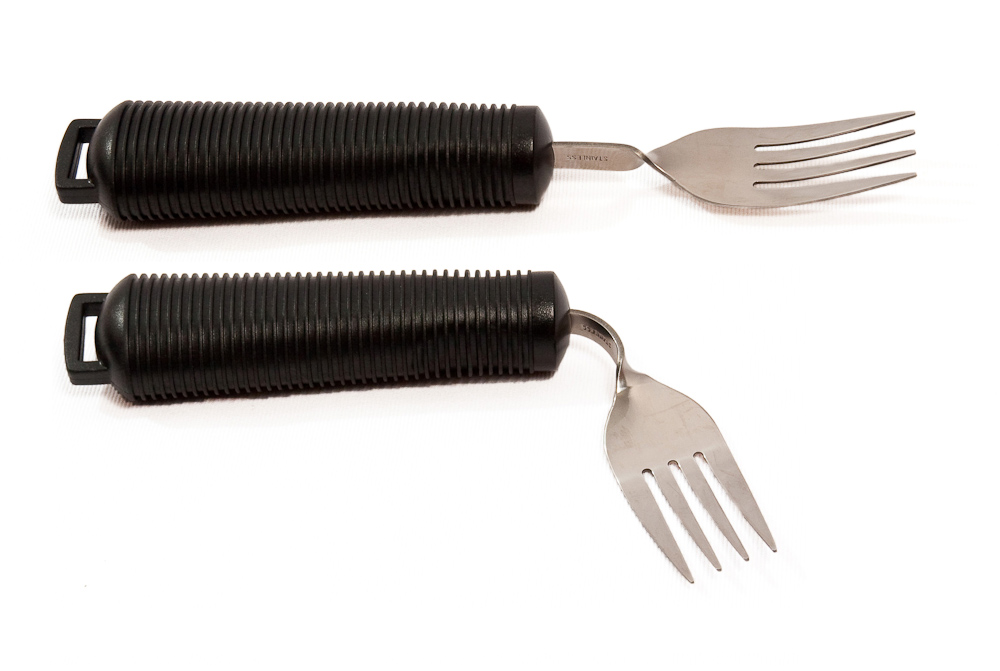
\includegraphics[width=5cm]{../figuras/talher.jpg}\\
			Fonte:\cite{vivere}
    
    \label{fig:talher}
  \end{center}
\end{figure}

A Figura \ref{fig:talher} mostra dois talheres que possuem cabos maiores para facilitar o manuseio, e um deles � ``dobrado'' para facilitar o posicionamento dos mesmos. Pacientes com quadros apresentados de Hemiplegia, Diplegia e algumas formas mistas podem se beneficiar com este tipo de talher.

}
\item{\acf{CAA}. Recursos eletr�nicos ou n�o para pessoas sem fala ou com limita��es dela (e.g., pranchas de comunica��o, vocalizadores, e softwares). A Figura \ref{fig:prancha} � um exemplo de prancha de comunica��o.

\begin{figure}[bth!]
  \begin{center}
    \caption{Exemplo de prancha de comunica��o}\vspace{.2cm}
			
      \centering
      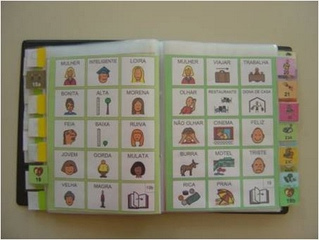
\includegraphics[width=5cm]{../figuras/prancha.jpg}\\
			Fonte:\cite{assistiva}
    
    \label{fig:prancha}
  \end{center}
\end{figure}

As pranchas de comunica��o exemplificadas na Figura \ref{fig:prancha} s�o meios de comunica��o para as pessoas com fala comprometida, isso pode ocorrer em todos os casos cl�nicos da \ac{PC}.

}
\item{Acessibilidade ao computador (e.g., teclados modificados, leitor de tela e ampliador de tela). A Figura \ref{fig:teclado} � um exemplo de teclado em modificado.
\vspace{-.5cm}
\begin{figure}[bth!]
  \begin{center}
    \caption{Exemplo de teclado em braile }\vspace{.2cm}
			
      \centering
      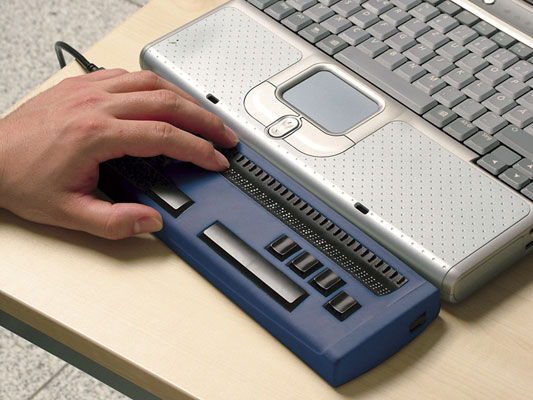
\includegraphics[width=4cm]{../figuras/teclado.jpg}\\
			Fonte:\cite{teclado}
    
    \label{fig:teclado}
  \end{center}
\end{figure}

A Figura \ref{fig:teclado} mostra que nos teclados modificados, a impress�o do que referencia cada tecla � na verdade um s�mbolo usado no alfabeto braile.

}
\item{Sistemas de controle de ambientes, que permitem que pessoas com dificuldades motoras controlem equipamentos a dist�ncia. A Figura \ref{fig:controle} � um exemplo de controle remoto para cegos.
\vspace{-.5cm}

\begin{figure}[bth!]
  \begin{center}
    \caption{Exemplo de controle assistivo}\vspace{.2cm}
			
      \centering
      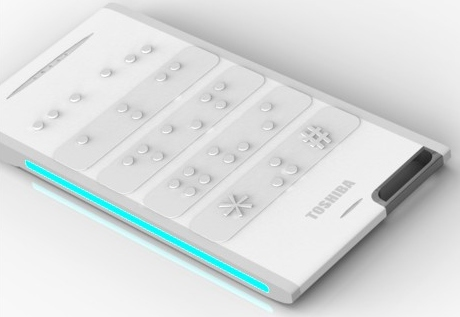
\includegraphics[width=4cm]{../figuras/controle.jpg}\\
			Fonte:\cite{controle}
    
    \label{fig:controle}
  \end{center}
\end{figure}
}
\vspace{-.5cm}
A Figura \ref{fig:controle} � um controle remoto que ao inv�s de possuir teclas com desenhos das fun��es e n�meros, os bot�es s�o representados em braile, para que os cegos possam manipular objetos a dist�ncia.

\item{Projetos Arquitet�nicos (e.g., cal�adas com guia para cegos e rampas de acesso). A Figura \ref{fig:rampa} � um exemplo de ramapa de acesso.

\begin{figure}[bth!]
  \begin{center}
    \caption{Exemplo de rampa de acesso}\vspace{.2cm}
			
      \centering
      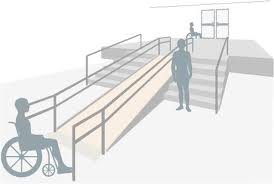
\includegraphics[width=4cm]{../figuras/rampa.jpg}\\
			Fonte:\cite{portal}
    
    \label{fig:rampa}
  \end{center}
\end{figure}

A Figura \ref{fig:rampa} representa uma rampa de acesso a cadeirantes, que torna poss�vel ao cadeirante o acesso a lugares mais elevados sem utilizar a ajuda de outras pessoas.

}
\item{�rteses e pr�teses, que permitem a troca ou ajuste de um membro. A Figura \ref{fig:protese} � um exemplo de pr�tese.
\vspace{-.5cm}
\begin{figure}[bth!]
  \begin{center}
    \caption{Exemplo de pr�tese}\vspace{.2cm}
			
      \centering
      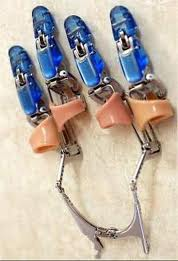
\includegraphics[width=3cm]{../figuras/protese.jpg}\\
			Fonte:\cite{protese}
    
    \label{fig:protese}
  \end{center}
\end{figure}
\vspace{-.5cm}
As pr�teses exemplificadas na Figura \ref{fig:protese}, ajudam as pessoas com membros danificados ou perdidos, a reabilita��o de movimentos.

}
\item{Equipamentos de aux�lio a postura (e.g., almofadas anat�micas e cintos). A Figura \ref{fig:cadeira} � um exemplo de cadeira de rodas com ajuste de postura.
\vspace{.5cm}
\begin{figure}[bth!]
  \begin{center}
    \caption{Exemplo de cadeira com regulagem de postura}\vspace{.2cm}
			
      \centering
      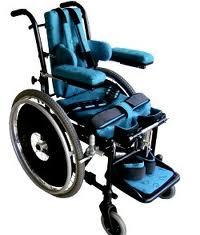
\includegraphics[width=4cm]{../figuras/cadeira.jpg}\\
			Fonte \cite{cadeira}
    
    \label{fig:cadeira}
  \end{center}
\end{figure}
}

Na Figura \ref{fig:cadeira} � poss�vel perceber o cinto na cadeira de rodas, que regulam a postura da pessoas do usu�rio.

\item{Equipamentos de mobilidade (e.g., cadeira de rodas motorizadas ou n�o e andadores). A Figura \ref{fig:cadeiramotorizada} representa um exemplo de cadeira de rodas motorizada.
\vspace{2cm}
\begin{figure}[bth!]
  \begin{center}
    \caption{Exemplo de cadeira de rodas motorizadas}
			
      \centering
      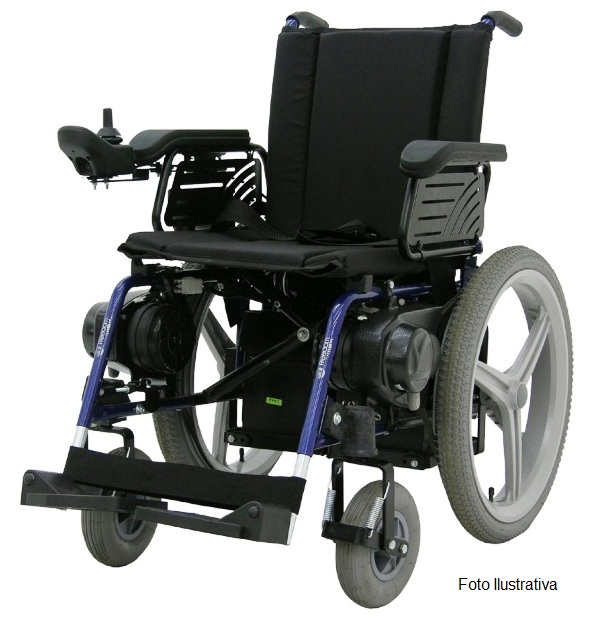
\includegraphics[width=3.5cm]{../figuras/cadeiramotorizada.jpg}\\
			Fonte: \cite{cinta}
    
    \label{fig:cadeiramotorizada}
  \end{center}
\end{figure}

Na Figura \ref{fig:cadeiramotorizada}, a cadeira possui um motor el�trico que faz com que a pessoa que a utiliza n�o necessite de grande esfor�o f�sico para moviment�-la.


}
\item{Aux�lio de surdos ou com audi��o parcial (e.g., aparelhos de surdez e telefones com teclado). A Figura \ref{fig:aparelhosurdez} � um exemplo de aparelho de surdez.
\vspace{-.5cm}
\begin{figure}[bth!]
  \begin{center}
    \caption{Exemplo de aparelho de surdez}
			
      \centering
      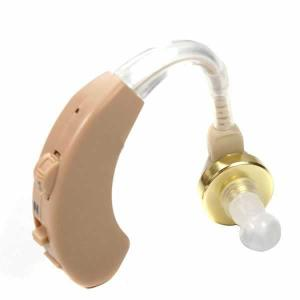
\includegraphics[width=3.5cm]{../figuras/aparelhosurdez.jpg}\\
			Fonte: \cite{surdez}
    
    \label{fig:aparelhosurdez}
  \end{center}
\end{figure}
}
\vspace{-.5cm}

Os aparelhos de surdez ilustrados pela Figura \ref{fig:aparelhosurdez} possibilitam que o �udio seja amplificado para que pessoas com defici�ncia auditiva parcial, possam escutar normalmente.

\item{Adapta��es a ve�culos. A Figura \ref{fig:carro} � um exemplo de carro adaptado a pessoas com defici�ncias f�sicas.
\begin{figure}[bth!]
  \begin{center}
    \caption{Exemplo de carro adaptado}\vspace{.2cm}
			
      \centering
      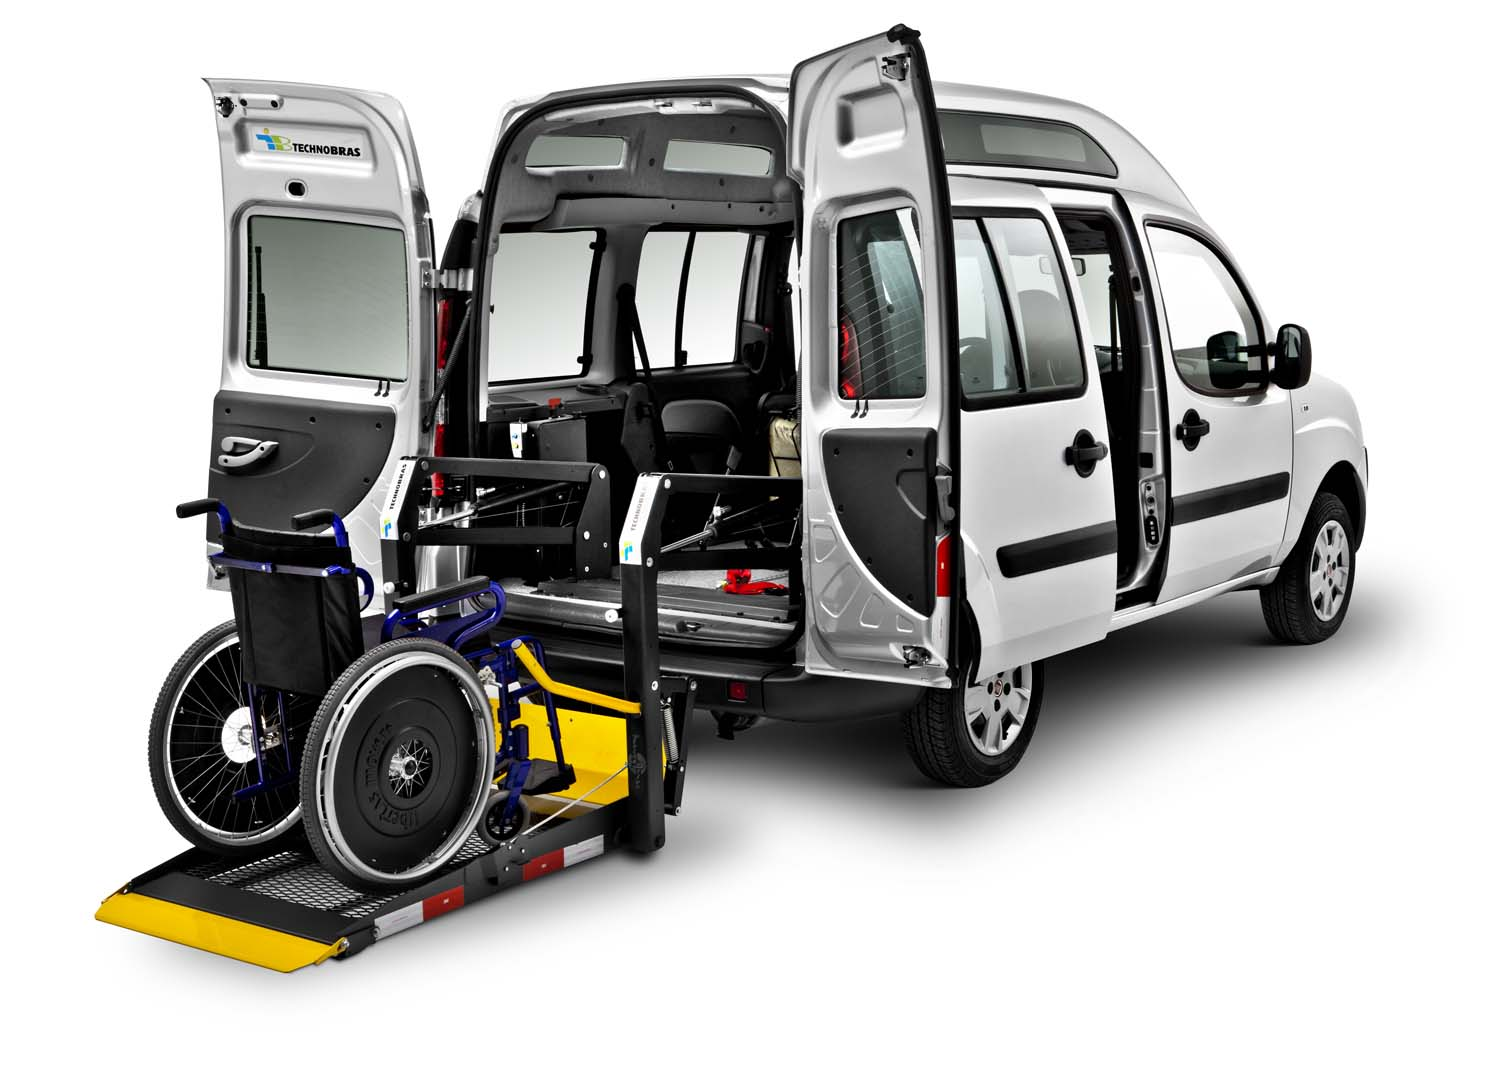
\includegraphics[width=4cm]{../figuras/carro.jpg}\\
			Fonte: \cite{fiat}
    
    \label{fig:carro}
  \end{center}
\end{figure}
}

A Figura \ref{fig:carro} � um exemplo de carro adaptado para pessoas com defici�ncia f�sica, possibilita que estas pessoas possam utilizar um ve�culo autonomamente.


\end{enumerate}


J� segundo a norma ISO 9999:2011(Anexo~\ref{iso9999}), a classifica��o das \ac{TA} se divide em categorias semelhante as diretrizes da \ac{ADA} por�m s�o mais espec�ficas. Para fins te�ricos, � utilizado no trabalho a classifica��o com base nas diretrizes da \ac{ADA} porque al�m da ISO 9999:2011 n�o incluir produtos e equipamentos usados exclusivamente por profissionais de sa�de e dispositivos implantados, a classifica��o \ac{ADA} apresenta um grupo de servi�os de \ac{TA} que promove o apoio � avalia��o da pessoa com defici�ncia, o desenvolvimento e personaliza��o de recursos, a integra��o da \ac{TA} com a��o e objetivos educacionais e de reabilita��o, e os apoios legais de concess�o \cite{corde}.


Uma pesquisa do \ac{W3C} \cite{wc} brasileiro aponta que das pessoas que usam aparelhos de \ac{TA}, 85\% � o computador o dispositivo mais usado, seguido do celular, {\it smarthphone} com 9\%, {\it tablet} com 2\%, e outros dispositivos com 4\%. Sendo cada vez mais necess�rio que existam op��es para esse tipo de p�blico dentro do acesso a informa��o.

A \ac{TA} faz parte da tecnologia, � a parte que auxilia a integra��o das pessoas que possuem algum tipo de defici�ncia. � uma �rea que envolve grandes por��es da popula��o, e que necessita de um cuidado especial, pois envolve al�m da pessoa com defici�ncia, as pessoas nos ambientes em que ela est� inserida.

\subsection{Legisla��o espec�fica de \acf{TA}}

Em rela��o a legisla��o de \ac{TA} alguns decretos s�o relevantes, entre eles a promulga��o do Decreto 3.298 
de 1999, que no artigo 19, fala do direito do cidad�o brasileiro com defici�ncia �s \ac{TA}. 
Nele consta que\cite{lima} (ver anexo {\ref{decreto1}}): 
\begin{quotation}
``Consideram-se ajudas t�cnicas, para os efeitos deste Decreto, os elementos que permitem 
compensar uma ou mais limita��es funcionais motoras, sensoriais ou mentais da pessoa 
portadora de defici�ncia, com o objetivo de permitir-lhe superar as barreiras da comunica��o e da 
mobilidade e de possibilitar sua plena inclus�o social. 
Par�grafo �nico. S�o ajudas t�cnicas:[...]elementos especiais para facilitar a comunica��o, a informa��o e a sinaliza��o para 
pessoa portadora de defici�ncia[...]``
\end{quotation}

O artigo 19 generaliza o termo Ajudas T�cnicas a todos os elementos que compensam limita��es do ser humano, por�m sem caracteriza��o ou classifica��o objetiva de tais ajudas. Tamb�m relevante, o decreto 5.296 de 2002, que d� prioridade de atendimento e estabelece normas gerais e crit�rios b�sicos para a promo��o da acessibilidade das pessoas com defici�ncia ou com 
mobilidade reduzida, possui um cap�tulo espec�fico sobre as ajudas t�cnicas no qual descreve 
v�rias inten��es governamentais na �rea da \ac{TA}, al�m de referir a constitui��o do 
\ac{CAT}. Neste decreto encontra-se que\cite{lima}: 
\begin{quotation}
``Consideram-se ajudas t�cnicas os produtos, instrumentos, equipamentos ou tecnologia 
adaptados ou especialmente projetados para melhorar a funcionalidade de pessoas portadoras de  
defici�ncia, com habilidade reduzida favorecendo autonomia pessoal, total ou assistida" .
\end{quotation}

No decreto 5.296\cite{cata} a legisla��o cita ao inv�s da compensa��o como no artigo 19, a autonomia total ou assistida das pessoas com defici�ncia. Embora esse Comit� leve a express�o ``Ajudas T�cnicas'' em sua 
denomina��o, tamb�m porque � a express�o prevista na legisla��o brasileira, 
os estudos desenvolvidos apontam e sugerem que as express�es 
``Tecnologia Assistiva'', ``Ajudas T�cnicas'' e ``Tecnologia de Apoio'', neste 
momento, continuem sendo entendidas como sin�nimos e que correspondam 
�s bases conceituais aprovadas pelo Comit�. Entretanto, estabelece a 
utiliza��o �nica da express�o ``Tecnologia Assistiva'' em seus documentos, 
como a mais apropriada, pelos seguintes motivos \apud{cata}{galvao}: 
\begin{itemize}
 
\item Por ser uma tend�ncia nacional j� firmada no meio acad�mico, nas 
organiza��es de pessoas com defici�ncia, em setores governamentais 
(Minist�rio MEC da Educa��o, Minist�rio da Ci�ncia e Tecnologia (MCT), Conselho Nacional de Desenvolvimento Cient�fico e Tecnol�gico CNPq), Institutos de Pesquisa (ITS Brasil) e no mercado de produtos; 
 
\item Pelo primeiro objetivo do Comit� de Ajudas T�cnicas, expl�cito no Artigo 
66 do Decreto 5296/2004, relativo � estrutura��o das diretrizes da �rea 
do conhecimento. A express�o Tecnologia Assistiva seria a mais 
compat�vel como a denomina��o de uma �rea de conhecimento, a ser 
oficialmente reconhecida; e
 
\item Por ser uma express�o bastante espec�fica ao conceito ao qual 
representa, diferentemente das express�es ``Ajudas T�cnicas'' e 
``Tecnologia de Apoio'', que s�o mais gen�ricas e tamb�m utilizadas para 
referirem-se a outros conceitos e realidades diferentes. 
\end{itemize}

Conforme votado e aprovado por unanimidade na quinta Reuni�o desse Comit�, al�m da determina��o de utiliza��o �nica da express�o Tecnologia Assistiva, foi decidido tamb�m que essa express�o seja utilizada no singular, por referir-se a uma �rea do conhecimento e sugere-se que se fa�am os poss�veis encaminhamentos para a revis�o da nomenclatura em 
instrumentos legais no pa�s. Este mesmo Comit� de Ajudas T�cnicas tamb�m aprovou, na sua terceira Reuni�o de abril de 2007, as bases conceituais que situam a Tecnologia Assistiva nos seguintes marcos \cite{cata,catb}: 

\begin{itemize}
\item �rea do Conhecimento;
\item Multidisciplinariedade;
\item Objetivos: promover a funcionalidade (atividade, participa��o) de 
pessoas com defici�ncia, mobilidade reduzida, ou idosas, visando sua 
autonomia, independ�ncia, qualidade de vida e inclus�o social; 
\item Composi��o: produtos, recursos, estrat�gias, pr�ticas, processos, 
m�todos e servi�os; e 
\item Ter presente os princ�pios do {\it Universal Design}\footnote{O conceito de Desenho Universal, ou ``{\it Universal Design}'', ou tamb�m chamado ``Desenho para todos'', � estudado a partir de alguns princ�pios tais como: equipara��o nas possibilidades de uso; flexibilidade no uso; uso simples e intuitivo; capta��o da informa��o; toler�ncia ao erro: m�nimo esfor�o f�sico; dimens�o e espa�o para uso e intera��o \cite{sepro}} e ITS BRASIL (Instituto de Tecnologia Social).

\end{itemize}

Apesar de uma iniciativa e uma legisla��o recente os assuntos acessibilidade e ajudas t�cnicas vem entrando no cotidiano dos brasileiros, pois h� uma cobran�a da parte governamental. Por�m, ainda existe uma defici�ncia em normas e na pr�pria legisla��o que regulamente as \ac{TA} principalmente na parte de classifica��o e exig�ncias.

\subsection{Iniciativas de \ac{TA}}
\label{iniciativas}

Existem v�rias iniciativas de \ac{TA} pelo mundo, como a  Funda��o SIDAR\cite{sidar} ({\it Seminario Iberoamericano sobre Diversidad y Accesibilidad en la Red}) que � uma institui��o de observa��o e recomenda��o na �rea da acessibilidade e inclus�o digital para os territ�rios ibero-americanos, a ATI\cite{ati} ({\it Assistive Technology Initiative}) na Universidade De George Mason na Virg�nia nos Estado Unidos, o INCNESI\cite{incnesi} (Iniciativa Nacional para os Cidad�os com Necessidades Especiais na Sociedade da Informa��o) que incentiva o uso de equipamentos para pessoas com defici�ncia em Portugal. 

Ainda no �mbito europeu, em 1999 foi organizado o Cons�rio \ac{EUSTAT} que desenvolveu um estudo entre 1997 e 1999, no contexto do Programa de Aplica��es Telem�ticas da Comiss�o Europeia, destinado a forma��o de usu�rios finais de \ac{TA}, envolvendo pessoas com defici�ncia ou idosos, seus familiares e profissionais assistentes pessoais, para que os mesmos pudessem fazer escolhas informadas, adequadas e respons�veis em rela��o a essas tecnologias. Esse estudo parte do princ�pio de que � fundamental a participa��o de usu�rio final como parceiro ativo na escolha das \ac{TA} que utiliza\cite{galvao}.

S�o parceiros do Cons�rcio \ac{EUSTAT} as seguintes organiza��es \cite{eustat}:

\begin{itemize}

\item SIVA {\it Servizio Informacione e Valutazione Ausili da Fondazione Dom Carlo Ghocchi Onlus}, da It�lia. Possui um centro de Inova��o e Transfer�ncia de Tecnologia, que incentiva projetos para autonomia de pessoas com defici�ncias;

\item CAPS  Centro de An�lise e Processamento de Sinais, do Instituto Superior T�cnico de Lisboa, Portugal;

\item \it{Association Nationale pour le Logement des personnes handicap�es}, da B�lgica;

\item \it{Groupement pour l�insertion des personnes handicap�es physiques}, da Fran�a;

\item \it{Danish Centre for Technical Aids for Rehabilitation and Education}, da Dinamarca; e

\item \it{Centro Studi Prisma}, da It�lia.

\end{itemize}

Os estudos que s�o parceiros do cons�rcio, s�o centros de refer�ncia em \ac{TA} na Europa, juntas s�o respons�veis por uma parte consider�vel de publica��es, dispositivos, sobre \ac{TA}. O Cons�rcio EUSTAT recomenda a classifica��o \ac{HEART} que prop�e tr�s grandes �reas de forma��o em 
rela��o �s \ac{TA}:
\begin{itemize} 
\item Componentes t�cnicos;
\item Componentes humanos; e
\item Componentes socioecon�micos.
\end{itemize}

Essa classifica��o tem ganhado for�a na atualidade, principalmente em decorr�ncia do paradigma inclusivo, o qual desloca as limita��es de funcionalidade e possibilidades de participa��o do �mbito restrito � defici�ncia em si, para situ�-las a partir das barreiras impostas pelo ambiente f�sico e social\cite{rodrigues}. Como n�o foi encontrado uma padroniza��o mundial para a defini��o de \ac{TA} as diferentes iniciativas encontradas se relacionam na tabela \ref{tabeladois}.

\begin{table}[bth!]
\centering
\scriptsize
\caption{Tabela com as diferen�as de Iniciativas de \ac{TA} encontradas.}\vspace{.2cm}
 \begin{tabular}{|p{2cm} |  p{3.9cm} | p{3cm} | p{4cm}| }
    \hline
    Pa�s & Termo Utilizado (Tradu��o) & Classifica��o & Defini��o \\ \hline
    Brasil & Tecnologia Assistiva, Ajudas T�cnicas &Ca\-te\-go\-ri\-as relativas aos e\-qui\-pa\-men\-tos & Melhorar as pessoas com defici�ncia e mobilidade re\-du\-zi\-da \\ \hline
    EUTSTAT & Ajudas T�cnicas e Tecnologia de Apoio & Classifica��o por componentes& Compensar as pessoas com defici�ncia e idosas \\ \hline
    ADA & {\it Assistive Technology} (Tecnologia Assistiva) & Trata as situa��es & Ajudas aos indiv�duos com defici�ncia em situa��es es\-pe\-c�\-fi\-cas \\ \hline	
		\end{tabular}
    \label{tabeladois}
		\\Fonte: o pr�prio autor.

\end{table}

A tabela {\ref{tabeladois}} mostra as diferen�as das tr�s iniciativas mais relevantes encontradas. Apesar da mudan�a de termos, as iniciativas n�o possuem grandes diferen�as entre si. A classifica��o da \ac{TA} � o �nico fator que diferencia nas iniciativas. Por�m, a relev�ncia da mudan�a � pequena, em rela��o a as ajudas �s pessoas com defici�ncia.


\section{Comunica��o Alternativa Ampliada (CAA)}

Na \ac{TA}, como mencionado anteriormente na se��o {\ref{Tecnologia Assistiva}} se divide em algumas classifica��es, dentro delas temos a \ac{CAA}, que � linha de pesquisa adotada neste trabalho. A \ac{CAA} abrange qualquer meio de comunica��o que suplemente ou substitua os m�todos naturais de fala ou escrita. � um meio que auxilia a comunica��o de um indiv�duo com outras pessoas. Os sistemas de \ac{CAA} podem ser divididos em pictoriais\footnote{Os sistemas pictoriais representam os referentes por analogia f�sica e n�o por conven��o arbitr�ria, o que lhes confere iconicidade e clareza denotativa, sendo bem compreendidos, aprendidos e lembrados por crian�as, estrangeiros e c�rebro-lesados. Contudo, o universo de significados que podem representar restringe-se ao imagin�vel \cite{fernando}.} e simb�licos\footnote{Os sistemas simb�licos representam referentes por conven��es arbitr�rias, usando regras de recombina��o e sintaxe espec�fica, o que resulta em opacidade denotativa, mas lhes permite representar virtualmente qualquer conceito, imagin�vel ou n�o \cite{fernando}.} podendo ser de alta tecnologia (e.g., sistemas computadorizados, e softwares especiais) e baixa tecnologia (e.g., simples, e n�o el�tricos) \cite{leydi}.

A \ac{CAA} � definida como uma maneira alternativa � comunica��o oral e escrita que compreende o uso de gestos, sinais manuais, express�es faciais, pranchas com s�mbolos pictogr�ficos, pranchas de alfabeto, comunicadores de voz gravada ou sintetizada at� sistemas sofisticados de computador \apud{glennen}{correia}. Inicialmente eram utilizados sistemas sem tecnologia, recorrendo apenas ao corpo humano, como a linguagem por sinais (e.g., libras) passando pelos sistemas anal�gicos ou de baixa tecnologia (e.g., cart�es e livros com s�mbolos e imagens) at� sistemas baseados em recursos computacionais (e.g., vocalizadores, e softwares para computador com s�ntese de voz) \apud{worthy}{correia}.

O trabalho da \ac{CAA} engloba uma s�rie de s�mbolos, recursos, estrat�gias e t�cnicas para auxiliar o desenvolvimento de uma comunica��o complementar. Os s�mbolos s�o as representa��es visuais, auditivas ou t�teis de um conceito; os recursos s�o os objetos ou equipamentos utilizados para transmitir as mensagens que podem ser pranchas de comunica��o, os comunicadores ou o computador; as t�cnicas s�o as formas como as mensagens s�o transmitidas e as estrat�gias referem-se ao modo como os recursos da \ac{CA} s�o utilizados \apud{king}{pelosi2}.

Como o foco deste trabalho � encontrar uma solu��o alternativa a pessoas que possuem defici�ncia na fala, em conjunto com defici�ncia motora (quadros tabela cl�nicos), a \ac{CAA} � a abordagem encontrada que melhor se encaixa neste contexto. Pois a \ac{CAA} utiliza estrat�gias e t�cnicas para o desenvolvimento de uma comunica��o complementar, que auxiliam a suplementa��o ou substitui��o da forma natural de comunica��o.


\section{Considera��es do Cap�tulo}

Com a pesquisa realizada no cap�tulo {\ref{cap:introducao}}, fica evidenciado que pessoas com necessidades especiais, precisam de recursos que supram ou compensem suas defici�ncias para que possam ser inseridas na sociedade. Apesar de uma por��o consider�vel da popula��o mundial possuir algum tipo de defici�ncia, os estudos e legisla��o sobre a \ac{TA} s�o consideravelmente recentes.
	
Al�m disso, vale ressaltar a import�ncia de que se desenvolva mais solu��es de \ac{TA}, principalmente acess�veis, e que os desenvolvedores, se preocupem com o ambiente em que esta pessoa est� inserida e as pessoas com as quais ela ir� interagir. Foram necess�rios conhecimentos sobre \ac{TA}, \ac{CAA} e acessibilidade para que se entenda o foco deste trabalho que visa encontrar uma solu��o alternativa de \ac{CAA} para pessoas que possuem \ac{PC} que apresentam defici�ncia motora e de fala.
	
Este trabalho se enquadra na Lei no 10.098, de dezembro de 2000 que estabelece crit�rios como o artigo 17 que garante direito de comunica��o e express�o por mecanismos, ou alternativas t�cnicas. Al�m disso, se enquadra tamb�m, no Decreto 5296/2004, Artigo 66 do Comit� de Ajudas T�cnicas, no qual estabelece o termo \acf{TA} como a denomina��o mais compat�vel ao tema.

O trabalho tamb�m pode ser classificado nas diretrizes da \ac{ADA} como um trabalho no contexto de \acf{CAA}. J� na norma ISO 9999:2011 na subcategoria, Produtos de Apoio para Treino de Comunica��o Alternativa e Aumentativa, c�digo 05 06 27, categoria Produtos de apoio para treino de comunica��o com imagens e desenhos.
     %chamada de arquivo introducao.tex
\setlength\abovedisplayskip{0pt} \setlength\belowdisplayskip{0pt}
\setlength\abovedisplayshortskip{0pt} \setlength\belowdisplayshortskip{0pt}

\chapter{Fundamenta��o Te�rica} \label{cap1}
Neste cap�tulo s�o apresentados os conceitos
b�sicos e a fundamenta��o te�rica necess�ria para o entendimento e abordagem do
problema do escalonamento de tripula��es.

\section{Programa��o Linear}

A programa��o linear consiste na modelagem e solu��o de problemas descritos com
uma fun��o objetivo linear sujeita a m�ltiplas restri��es lineares. A forma
gen�rica de um problema de programa��o linear �\cite{dantzig1955generalized}:

\begin{align} \label{funcao_obj} \text{maximizar} \: z &= \sum_{j=1}^{p}
    c_jx_j, \intertext{sujeito �:} \label{restricoes} \sum_{j=1}^{p} a_{ij} x_j
    \leq b_i, i &= 1, 2, \ldots, q \\ \label{restricoes_triviais} x_j \geq 0, j
    &= 1, 2, \ldots, p, \end{align}.

Onde $c_j, a_{ij}$ e $b_i$ s�o n�meros reais que definem o problema e $x_j$
para $j=1, 2, \ldots, p$ s�o as vari�veis de decis�o. A
fun��o~\eqref{funcao_obj} � denominada de fun��o objetivo, a qual deve ser
maximizada. Note que o m�ximo de $f(x)$ � o m�nimo de $-f(x)$ com o sinal
oposto max $f(x) = - \text{min} f(x)$. As inequa��es em~\eqref{restricoes}
representam um conjunto de $q$ restri��es lineares que restringem o espa�o de
busca para um poliedro convexo. O m�ximo da fun��o deve estar contido dentro
deste poliedro. As desigualdades em~\eqref{restricoes_triviais} s�o denominadas
de restri��es triviais ou de n�o negatividade.

Cada restri��o em~\eqref{restricoes} pode ser convertida para restri��o de
igualdade utilizando-se uma vari�vel extra, denominada de vari�vel de folga. A
utiliza��o d�-se por:

\[ \label{restricoes} \sum_{j=1}^{p} a_{ij} x_j \leq b_i \Leftrightarrow
\begin{cases} \Sigma_{j=1}^{p} a_{ij} x_j + x_{p+i} = b_i\\ x_{p+i} \geq 0
\end{cases} \].

� poss�vel ainda utilizar duas igualdades para representar uma igualdade:

\[ \label{restricoes} \sum_{j=1}^{p} a_{ij} x_j = b_i \Leftrightarrow
\begin{cases} \Sigma_{j=1}^{p} a_{ij} x_j \leq b_i\\ \Sigma_{j=1}^{p} a_{ij}
x_j \geq b_i \end{cases} \]

Para um problema qualquer de programa��o linear com restri��es de desigualdades
e igualdades, sempre � poss�vel reestrutur�-lo atrav�s da adi��o de vari�veis
de folga, para que o problema passe a ter apenas igualdades. Portanto, todo e
qualquer problema de programa��o linear pode ser expresso como:

\begin{align} \label{fo} \text{maximizar} \: z &= \sum_{j=1}^{n} c_jx_j
    \intertext{sujeito �:} \label{res} \sum_{j=1}^{n} a_{ij} x_j \leq b_i, i &=
    1, 2, \ldots, m \\ \label{res_t} x_j \geq 0, j &= 1, 2, \ldots, n
    \intertext{que � equivalente �:} \label{fo2} \text{maximizar} \: z &= cx
\intertext{sujeito �:} \label{res2} Ax &= b \\ \label{res_t2} x &\geq 0,
\end{align}.

Onde $c^T \in \mathbb{R}^n$, $x \in \mathbb{R}^n$, $b \in \mathbb{R}^m$, $A \in
\mathbb{R}^{m \times n}$ e $a_j \in \mathbb{R}^m$.

Baseado nas restri��es~\eqref{res2} e~\eqref{res_t2}, pode-se descrever o
problema como encontrar $x \in X$, onde $X = \{ x \in \mathbb{R}^n | Ax = b, x
\geq 0 \}$, tal que $cx$ seja maximizado. Ao conjunto $X$ d�-se o nome de
regi�o fact�vel ou espa�o de busca. Para um $x \in X$ qualquer, diz-se que $x$
� uma solu��o fact�vel.  Para um $x^* \in X$, se $cx^* \geq cx \forall x \in
X$, ent�o $x^*$ � a solu��o �tima do problema. O espa�o de busca para um
problema de programa��o linear � sempre um poliedro convexo, se interpretado
geometricamente, e a solu��o �tima para o mesmo sempre est� em um v�rtice do
poliedro.

Um problema de programa��o linear pode ser ainda expresso em uma forma
matricial, ou em forma de conjunto. Suas representa��es s�o respectivamente:

\begin{align} \label{lp_fo} \text{maximizar} \: z &= cx \intertext{sujeito �:}
\label{lp_r} Ax &= b \\ \label{lp_tr} x &\geq 0 \intertext{} \label{lp_set}
\text{max } \{ cx : Ax &\leq b, x \geq 0 \} \end{align}

\subsection{M�todos de solu��o}

Considerando o conjunto $X$ descrito na se��o anterior, o objetivo de efetuar a
modelagem de um problema utilizando-se programa��o linear � utilizar recursos
matem�ticos e algor�tmicos para resolver o modelo, e por conseguinte o problema
original. Esta se��o apresenta os tr�s principais m�todos encontrados na
literatura durante o desenvolvimento deste trabalho: o m�todo simplex; o m�todo
dos elipsoides; o m�todo do ponto interior.

O m�todo Simplex~\cite{dantzig1990origins} foi apresentado em 1947 por George
B. Dantzig com o objetivo de resolver o problema de programa��o linear. O
m�todo consiste em encontrar uma solu��o fact�vel ao problema, e iterativamente
mover para uma solu��o melhor ou igual que a atual. Considerando que a solu��o
est� em um v�rtice do poliedro, � necess�rio apenas explorar os v�rtices. Tendo
em vista que existe um n�mero finito de v�rtices para um poliedro descrito por
um conjunto finito de restri��es lineares (que geometricamente correspondem a
hiperplanos), fica claro que o simplex converge em um n�mero finito de passos.
Apesar de que na m�dia o simplex resolve o problema em um n�mero polinomial de
passos, em 1972 foi apresentado uma prova de que o m�todo simplex no seu pior
caso � exponencial~\cite{klee1972good}.  Klee e Minty apresentaram um politopo
especialmente projetado para que o m�todo simplex leve um n�mero exponencial de
passos, o politopo � denominado de Cubo de Kleen-Minty.

Em decorr�ncia da descoberta do cubo de Klee-Minty, diversos pesquisadores
iniciaram um estudo em busca de um m�todo capaz de resolver o problema de
programa��o linear em tempo polinomial. Um dos primeiros trabalhos apresentados
na literatura propondo um algoritmo polinomial foi o m�todo dos
elipsoides~\cite{khachian}. O m�todo consiste em criar um elipsoide que englobe
a solu��o �tima e reduzi-lo sequencialmente de modo que a solu��o �tima sempre
esteja dentro do elipsoide. O m�todo possui, em teoria, converg�ncia garantida
em tempo polinomial. No entanto, na pr�tica o m�todo apresenta um desempenho
inferior ao simplex, como problemas de instabilidade num�rica. O m�todo
dos elipsoides demonstrou que diversos problemas podem ser resolvidos em tempo
polinomial~\cite{Grotschel1981}.

Em 1984 foi proposto um novo m�todo polinomial para a solu��o do problema da
programa��o linear, denominado de m�todo do ponto interior\cite{potra2000interior}.
Este m�todo consiste em a partir de uma solu��o fact�vel centro do politopo, perturba-la
at� que a mesma convirja para o ponto �timo. O m�todo do ponto interior tamb�m �
referenciado na literatura como m�todo das barreiras, j� que as restri��es
lineares s�o reescritas como fun��es assint�ticas que tendem ao infinito quando
a restri��o linear original � violada. O m�todo do ponto interior apresentou um
desempenho compar�vel ao do simplex, e � especialmente aplicado em problemas de
larga escala.


\subsection{Dualidade}

Considerando o problema de programa��o linear apresentado
em~\eqref{funcao_obj},~\eqref{restricoes} e~\eqref{restricoes_triviais}, que a
partir de agora ser� denominado de problema primal,

\begin{align} \text{maximizar} \: z = \sum_{j=1}^{p} c_jx_j, \intertext{sujeito
a:} \label{rp} \sum_{j=1}^{p} a_{ij} x_j \leq b_i, i = 1, 2, \ldots, q \\
\label{} x_j \geq 0, j = 1, 2, \ldots, p, \end{align}.

O problema dual � constru�do atribuindo-se uma vari�vel $u_i, i = 1, 2, \ldots,
q$ a cada restri��o em~\eqref{rp} e definindo o problema como:

\begin{align} \text{minimizar} \: d = \sum_{i=1}^{q} b_iu_i, \intertext{sujeito
a:} \label{} \sum_{i=1}^{q} a_{ij} u_i \leq c_j, i = 1, 2, \ldots, p \\
\label{} u_i \geq 0, i = 1, 2, \ldots, q, \end{align}

O problema primal e dual em sua forma matricial s�o dados por:

\begin{align} \label{} \text{maximizar} \: z &= cx \intertext{sujeito �:}
    \label{prnt} Ax &= b \\ \label{prt} x &\geq 0, \intertext{e} \label{}
    \text{minimizar} \: d &= ub \intertext{sujeito �:} \label{drnt} uA^t &= c \\
    \label{drt} u &\geq 0,
\end{align}

� partir do problema primal e dual, conforme demonstrado
em~\cite{maculan2006otimizaccao}, segue que:

\begin{enumerate} \label{x} \item Se $\overline{x}$ satisfaz~\eqref{prnt}
        e~\eqref{prt} e $\overline{u}$ satisfaz~\eqref{drnt} e~\eqref{drt},
    ent�o $c\overline{x} \leq \overline{u}b$; \item Se $\overline{x}$ e
        $\overline{u}$ forem \textbf{solu��es fact�veis} do problema primal e dual,
        respectivamente, e $c\overline{x} = \overline{u}b$, ent�o
        $\overline{x}$ � a \textbf{solu��o �tima} do problema primal e $\overline{u}$ �
        a solu��o �tima do problema dual;
    \item Se $\tilde{x}$ � a \textbf{solu��o �tima} do problema primal e $\tilde{u}$ � a
        \textbf{solu��o �tima} do problema dual, ent�o $c\tilde{x} = \tilde{u}b$.
\end{enumerate}

O primeiro item � conhecido como teorema da \textbf{dualidade fraca}, e sua implica��o �
que uma solu��o dual � um limite superior de otimalidade para o problema
primal.  O segundo e terceiro item constituem o teorema da \textbf{dualidade forte}, que
pode ser utilizado para provar que uma solu��o de um problema primal � a �tima.

\section{Programa��o Linear Inteira}

A Programa��o Linear Inteira (PLI)~\cite{wolsey1998integer} trata de modelar problemas onde existem
vari�veis inteiras. A forma gen�rica de um problema d�-se de forma an�loga a de
um problema de programa��o linear:

\begin{align} \text{} \: z = \sum_{j=1}^{p} c_jx_j, \intertext{sujeito �:}
\label{} \sum_{j=1}^{p} a_{ij} x_j \leq b_i, i &= 1, 2, \ldots, q \\
\label{interg} x_j \geq 0 \text{ e } x_j \in \mathbb{Z}, j &= 1, 2, \ldots, p,
\end{align}

Nota-se que o modelo acima � exatamente igual a um problema gen�rico de
programa��o linear, exceto pela restri��o em~\eqref{interg}, que faz com que os
valores de $x_j$ sejam inteiros. Esta restri��o � denominada de restri��o de
integralidade.

Outros problemas podem precisar de solu��es que sejam inteiras e fracion�rias, estes
problemas s�o denominados de problemas de programa��o linear mista (PLIM) e
possuem uma forma gen�rica de:

\begin{align} \text{} \: z = \sum_{j=1}^{p} c_jx_j, \intertext{sujeito �:}
    \label{plim_r} \sum_{j=1}^{p} a_{ij} x_j \leq b_i, i &= 1, 2, \ldots, q \\
    \label{plim_v} \sum_{j=1}^{r} g_{ij} y_j \leq d_i, i &= 1, 2, \ldots, q \\
    \label{} x_j \geq 0, j &= 1, 2, \ldots, p, \\ \label{plim_int} y_j \geq 0
\text{ e } y_j \in \mathbb{Z}, j &= 1, 2, \ldots, r \end{align}

A restri��o~\eqref{plim_r} representa as vari�veis fracion�rias do modelo, a
restri��o~\eqref{plim_v} as vari�veis inteiras e~\eqref{plim_int} � a restri��o
de integralidade.

Existem ainda problemas na qual � utilizado apenas vari�veis bin�rias, a estes
problemas d�-se o nome de problema de programa��o linear inteira bin�ria
(PLIB).  Eles possuem a forma gen�rica de:

\begin{align} \text{} \: z = \sum_{j=1}^{p} c_jx_j, \intertext{sujeito �:}
\label{} \sum_{j=1}^{p} a_{ij} x_j \leq b_i, i &= 1, 2, \ldots, q \\
\label{pbin} x_j \in \{0, 1\}, j &= 1, 2, \ldots, p, \end{align}

As restri��es s�o iguais a de um problema de programa��o linear, exceto para a
restri��o~\eqref{pbin}, que restringe o dom�nio das vari�veis para valores de
$0$ ou $1$.

A PLI e suas variantes (PLIM e PLIB) s�o problemas $\mathcal{NP}$-completos,
conforme demonstrados por~\cite{karp1972} e~\cite{papadimitriou1981complexity}.
Sabe-se ainda que a PLI � um problema $\mathcal{NP}$-completo forte, portanto, �
improv�vel que exista um algoritmo pseudo-polinomial capaz de
resolv�-lo~\cite{garey1978strong}.

Considere o problema de PLI a seguir:

\begin{equation} \label{pli_example} A = \begin{pmatrix} -1 &  2 \\ 5 &  1 \\
    -2 & -2 \end{pmatrix}, \quad b = \begin{pmatrix} 4 \\ 20 \\ -7
        \end{pmatrix}, \quad c^T = \begin{pmatrix} 1 \\ 1 \end{pmatrix}
\end{equation}


\begin{figure}[!htb]
    \centering
    \begin{minipage}{.48\textwidth}
        \centering
        \begin{tabular}{r l}
            fun��o objetivo & = $6.9090\ldots$ \\
            $x_1$           & = $3.2727\ldots$ \\
            $x_2$           & = $3.6363\ldots$
        \end{tabular}
        \captionof{table}{Solu��o da PLI}
        \label{rrrr}
    \end{minipage}
%
    \begin{minipage}{0.48\textwidth}
        \centering
        \includegraphics[width=1\linewidth]{../figuras/pli.pdf}
        \caption{Espa�o de busca do problema \eqref{pli_example}}
        \label{espacobusca}
    \end{minipage}
\end{figure}

Resolvendo-o obt�m-se o resultado apresentado na figura~\ref{rrrr}.
Considerando que o problema de PLI admite apenas vari�veis com valores
inteiros, o resultado acima � inv�lido como resposta para o problema.
Observando-se a figura~\ref{espacobusca}, que cont�m o espa�o de busca do problema
em quest�o, pode-se observar que os pontos que s�o fact�veis ao problema de PLI
s�o um subconjunto do espa�o de busca de um problema de programa��o linear com
as mesmas restri��es. Observa-se ainda que a solu��o �tima do problema de PLI
n�o coincide com a solu��o �tima do problema de programa��o linear. Portanto,
torna-se necess�rio a utiliza��o de m�todos espec�ficos para resolver problemas de PLI.

\subsection{Relaxa��o Linear}

O conceito de relaxa��o no contexto de otimiza��o corresponde a remover alguma
restri��o do problema. O relaxamento de um problema tem como objetivo torn�-lo
mais f�cil de resolver. Dentre as diversas restri��es que podem ser relaxadas, uma delas
� a restri��o de integralidade, que se removida leva a uma relaxa��o linear.
Considerando que o problema de PLI gen�rico � $\mathcal{NP}$-completo, a
relaxa��o linear torn�-lo um problema $\mathcal{P}$, que pode ser resolvido mais
rapidamente\cite{garey1978strong}.

Seja $x^*$ a solu��o �tima de um problema de maximiza��o PLI e $\hat{x}^*$ a
solu��o �tima da relaxa��o do mesmo, segue que $x^* \leq \hat{x}^*$. Portanto a
relaxa��o linear � um limite superior de otimalidade para um problema de PLI
qualquer. O mesmo � v�lido para PLIM e PLIB.

O espa�o de busca de um problema de PLI consiste em um conjunto de pontos com
coordenadas inteiras. A figura~\ref{espacobusca} cont�m o conjunto de pontos
que satisfazem o problema original. O contorno que envolve os pontos consiste
na relaxa��o linear, onde a restri��o de integralidade foi desconsiderada.
Pode-se notar que a �rea de busca aumentou e a solu��o �tima da relaxa��o �
maior do que o problema original.

\subsection{Relaxa��o Combinat�ria}

Para problemas combinat�rios (discretos), a relaxa��o combinat�ria consiste em
remover uma ou mais restri��es de um problema. Igualmente a relaxa��o linear, a
relaxa��o combinat�ria oferece um limite superior de otimalidade para um
problema de PLI, no entanto a relaxa��o combinat�ria n�o necessariamente torna
o problema mais f�cil de se resolver, no sentido de diminuir a complexidade.

Um exemplo de relaxa��o combinat�ria � a remo��o da restri��o de sub-tours no
problema do caixeiro viajante, que transforma-o em um problema de designa��o. O
problema de designa��o � um problema $\mathcal{P}$. Na pr�tica utiliza-se esta
relaxa��o para resolver-se o problema do caixeiro
viajante~\cite{laporte1992traveling}.

\subsection{M�todos de solu��o de PLI}

Um dos primeiros m�todos para solu��o de problemas de programa��o inteira foi
proposto por~\cite{gomory1960solving,gomory1960algorithm}. O m�todo veio a ser
denominado de m�todo de planos de cortes, que consiste em gerar hiperplanos
(restri��es) que removem o ponto �timo da relaxa��o linear sem remover o �timo
da PLI. Esta sequencia de cortes faz com que a solu��o �tima da relaxa��o linear
seja a mesma do problema original.

Utilizando-se planos de corte pode-se
resolver problemas de PLI apenas com o SIMPLEX. O m�todo funciona teoricamente,
por�m na pr�tica o m�todo apresenta problemas de instabilidade num�rica,
tornando-o invi�vel. Existem estudos que propuseram mudan�as para viabilizar
o m�todos~\cite{cook2009numerically}. \cite{zanette2011lexicography} apresenta
o uso do simplex lexicogr�fico para evitar a instabilidade num�rica. Outro
plano de corte bem estabelecido na literatura � o corte por arredondamento
inteiro misto~\cite{wosley88}, que foi demonstrado ser uma forma gen�rica para
planos de cortes. Apesar de sua inviabilidade, os planos de corte possuem grande
import�ncia te�rica.

\cite{little1963algorithm} e
\cite{land2010automatic} propuseram um m�todo de enumera��o impl�cita que veio a
ser chamado de \textit{Branch and Bound}(BnB). O BnB consiste em dividir um
espa�o de busca $S$ em subespa�os $S_1, S_2, \ldots, S_n$ de modo que
$S_1 \cup S_2 \cup \ldots \cup S_n = S$. Para cada espa�o gerado � calculado
um limite superior e inferior de otimalidade, e os espa�os s�o divididos
novamente. Baseado nos limites, o BnB tende a seguir por regi�es que levam
a melhores resultados e elimina regi�es infrut�feras. Um exemplo de
limite superior � a relaxa��o linear, e um limite inferior � qualquer solu��o
fact�vel para um problema. Se uma regi�o $S_1$ possui um limite inferior de
$z = 22.4$ e uma regi�o $s_2$ possui limite superior de $z = 21.0$, esta regi�o pode
ser descartada desde que seja encontrado uma solu��o fact�vel em $S_1$.
O desempenho do BnB est� diretamente ligado � dist�ncia entre os limites inferiores
e superiores, quanto menor a dist�ncia melhor o desempenho tende a ser.

Uma das caracter�sticas dos planos de corte, � que eles podem reduzir a
dist�ncia entre a solu��o �tima da relaxa��o linear e a solu��o �tima
da PLI. Sendo assim, pode-se incluir a gera��o de planos de cortes no processo
de solu��o do BnB, melhorando assim seus limites. O BnB que utiliza planos de
cortes � denominado de \textit{Branch and Cut} (BnC).

\section{Problemas com muitas restri��es ou vari�veis}

Na programa��o linear inteira existem problemas que tornam-se invi�veis de serem
resolvidos puramente com os m�todos acima mencionados. Tomemos o problema
do caixeiro viajante(TSP) como exemplo. Em~\eqref{stsp} pode-se observar uma das
muitas poss�veis modelagens para o problema do TSP. A restri��o~\eqref{stsp3} �
o que difere o TSP de um problema de designa��o, e � o que torna o TSP um
problema $\mathcal{NP}$-dif�cil, pois esta restri��o insere uma quantidade
fatorial de restri��es no modelo do TSP. Em~\eqref{fat_tsp} temos uma f�rmula
que descreve o n�mero de restri��es que~\eqref{stsp3} insere. Portanto,
� necess�rio que se utilize um procedimento denominado de gera��o de planos de cortes
para lidar com esta grandeza de restri��es.

\begin{equation} \label{fat_tsp}
    \sum_{k=2}^{|A|-1} \binom{|A|}{k}!
\end{equation}


\begin{subequations}
    \label{stsp}
    \begin{align} \label{func_tsp2}
        z &= min \sum_{(i,j) \in A} c_{ij}x_{ij}
        \intertext{sujeito �:}
        & \sum_{i \in V}     x_{ij} =  1          & \forall    j \in V, i \neq j                   & \label{stsp1} \\
        & \sum_{j \in V}     x_{ij} =  1          & \forall    i \in V, i \neq j                   & \label{stsp2} \\
        & \sum_{(i,j) \in A} x_{ij} = |S|-1       & \forall \; S \subset V, 2 \leq |S| \leq |V|-1  & \label{stsp3} \\
        & 0 \leq x_{ij} \leq 1                    & \forall    (i,j) \in E                         &
    \end{align}
\end{subequations}

Considerando o modelo gen�rico de PLI~\eqref{glinhas} a seguir:

\begin{subequations} \label{glinhas}
    \begin{align} \label{}
        \text{maximizar} \: z &= cx
        \intertext{sujeito �:}
        \label{} Ax &= b \\
        \label{} x &\geq 0
    \end{align}
\end{subequations}

Pode-se escolher um conjunto arbitr�rio de restri��es tal que
$\tilde{A} \subseteq A$ e $\tilde{b} \subseteq b$,
formando um novo problema de PLI~\eqref{glinhas2}.

\begin{subequations} \label{glinhas2}
    \begin{align} \label{}
        \text{maximizar} \: z &= cx
        \intertext{sujeito �:}
        \label{} \tilde{A}x &= \tilde{b} \\
        \label{} x &\geq 0
    \end{align}
\end{subequations}

Tem-se que~\eqref{glinhas2} � o problema apresentado em~\eqref{glinhas}, por�m com um conjunto
reduzido de restri��es, que pode ser resolvido mais facilmente. No entanto,
a solu��o �tima $\tilde{x}^*$ n�o necessariamente ir� satisfazer
a~\eqref{glinhas}. Ent�o � necess�rio que verifique-se qual das restri��es
s�o violadas e estas devem ser inseridas em~\eqref{glinhas2}, que deve ser
resolvido novamente. Este verifica��o � conhecido como problema da separa��o,
que � $\mathcal{NP}$-completo, conforme demonstrado
em~\cite{nemhauser1988integer}.

O problema da separa��o pode ser formulado como outro problema de PLI, formulado de
modo dual, que indica qual � a restri��o mais violada dentre todas. Esta
restri��o � ent�o adicionada ao problema, que � re-otimizado e pode ter
outras vari�veis violadas. O processo � repetido at� que n�o existam mais
vari�veis violadas.

A principal vantagem deste m�todo � que o conjunto de restri��es finais �
muito menor do que o total de restri��es do problema original. E portanto, o
custo de resolver diversos problemas de separa��o e efetuar m�ltiplas
re-otimiza��es do problema original tende a ser mais r�pida do que resolver
o problema original.

Existem ainda problemas onde o n�mero de restri��es � relativamente pequeno,
enquanto que o \textbf{n�mero de vari�veis � muito maior}. Um exemplo de problema com
este comportamento � o \textit{Cutting stock problem}. O problema consiste
em dado uma demanda de pe�as de tamanhos arbitr�rios e um estoque de pe�as de
tamanho fixo, determinar como cortar o estoque para obter as pe�as demandadas
com um desperd�cio m�nimo. Sua formula��o � dada a seguir:

\begin{subequations}\label{cuttingsp}
    \begin{align}
        z = min \sum_{j \in J} c_{j}x_{ij} \\
        \sum_{j \in J} a_{ij} x_j \geq b_j, \forall i \in I \\
        x_j \in \mathbb{Z}^+
    \end{align}
\end{subequations}

Onde $c_j$ corresponde a sobra de utilizar-se o corte $j$, $b_i$ � a demanda
para pe�as do tipo $i$, e $a_{j}$ corresponde a um padr�o de corte.
Considere o seguinte exemplo: Deseja-se pe�as de tamanho $3, 4, \text{e } 5$
cortados a partir de um tubo de tamanho $10$. Alguns padr�es v�lidos de corte
s�o: $(5, 5)$, $(5, 4)$, $(3, 3, 3)$, etc.

A matriz $A$ ter� dimens�es $m \times n$, onde $m$ � o n�mero de diferentes
pe�as que s�o necess�rios e $n$ � o total de combina��es de como se pode
efetuar os cortes. Conforme se aumenta o valor de $m$, $n$ cresce
exponencialmente.

Considerando que no simplex o n�mero de vari�veis b�sicas � limitado pelo
n�mero de restri��es, em um problema onde existe uma quantidade muito maior
de colunas do que linhas boa parte do tempo de solu��o seria gasto processando
vari�veis que ao fim teriam o seu custo fixado em $0$. Portanto, a maioria
das colunas n�o s�o necess�rias para obter-se o resultado final do problema.

A solu��o de problemas com muitas vari�veis funciona de modo an�logo ao com
muitas restri��es. Com base no problema original, � formulado um novo problema,
denominado de problema mestre, que cont�m apenas um conjunto reduzido de colunas
do problema original. A relaxa��o do problema mestre � resolvido e obt�m-se os
pre�os duais, que s�o utilizados para determinar quais colunas s�o necess�rias
para resolver o problema at� seu ponto �timo. O problema auxiliar que � capaz
de determinar quais colunas s�o necess�rias, � denominado de subproblema. No
capitulo~\ref{chap3} o problema mestre e o subproblema s�o apresentados
formalmente.

Utilizando-se a solu��o �tima $\tilde{x}^*$ do problema reduzido e sua solu��o
�tima dual $\tilde{y}^*$ pode-se testar $\tilde{y}^*$ por restri��es violadas
no problema dual completo. Portanto, adicionar restri��es no problema dual
corresponde a adicionar colunas (e vari�veis) no problema primal. Este processo
de resolver o problema primal reduzido e detectar restri��es duais pode ser
repetido at� que se obtenha uma solu��o $\tilde{x}^*$ que n�o viole restri��es
no problema dual.

Neste capitulo foi apresentado os principais conceitos te�ricos necess�rios para
o entendimento do problema a ser abordado nos pr�ximos cap�tulos deste trabalho.
Discutiu-se as principais representa��es de problemas de programa��o linear e
programa��o linear inteira, suas principais propriedades e m�todos de solu��o.
Por fim introduziu-se o conceito de utilizar custo reduzido e o problema dual
para determinar restri��es violadas ou colunas que podem melhorar a fun��o objetivo.

\chapter{O problema de cobertura, particionamento e escalonamento de tripula��o}
\label{chap3}

A aloca��o de tripula��o (CSP) consiste de um dos principais problemas de planejamento
de opera��es dentro do contexto de empresas de transporte a�reo e terrestre.
Segundo reportado por~\cite{zeren2012improved}, os gastos com tripula��o consistem
na segunda maior fonte de despesas, atr�s apenas dos gastos de combust�veis. Portanto,
de um ponto de vista operacional pode-se utilizar m�todos de otimiza��o para oferecer
redu��es significativas nos gastos, enquanto que de um ponto de vista acad�mico � um
problema dif�cil de resolver, com grandes inst�ncias e uma aplicabilidade pr�tica.

O CSP pode ser definido como criar e designar jornadas para um conjunto de tripulantes de
modo a cobrir todas as tarefas que devem ser realizadas. Conforme j� definido no
cap�tulo~\ref{cap1}, uma \textbf{tarefa} � definida como sendo uma a��o que deve
ser realizada por uma tripula��o. Durante uma tarefa a tripula��o dedica-se integralmente
a mesma durante um per�odo de tempo fixo. Uma \textbf{jornada} consiste em um conjuntos de
tarefas que dever ser cobertas por uma tripula��o. A cada jornada � atribu�do um
custo operacional, e a gera��o de jornadas esta limitada por leis trabalhistas e
sindicais. O principal objetivo do CSP � determinar o conjunto de jornadas que
cobre todas as tarefas, reduzindo o custo operacional, respeitando as restri��es
impostas em rela��o as jornadas de trabalho e designando apenas uma tripula��o
por jornada.

Conhecendo-se um n�mero suficientemente grande de jornadas (grande o suficiente
para poder cobrir todas as tarefas de modo fact�vel) pode-se modelar o CSP como
um problema de \textit{set covering problem} (SCP) ou \textit{set partitioning problem} (SPP),
dependendo se � desej�vel que uma jornada seja coberta mais de uma vez. No restante
deste capitulo � discutido os problemas de cobertura e particionamento assim como uma
abordagem mais detalhada do CSP.

\section{Problema de Escalonamento de Tripula��o}
\label{csppppp}

Esta se��o � dedicada a explicar a modelagem e as inst�ncias utilizadas neste
trabalho. Utilizou-se as inst�ncias presentes na \textit{OR-Library}~\cite{beasley1990or},
apresentadas inicialmente em~\cite{beasley1996tree}. Este trabalho utiliza a vers�o
de Junho de 2016 das inst�ncias.

Na \textit{OR-Library} existem 10 problemas de CSP presentes, sendo que todos
eles s�o utilizados como objeto de estudo neste trabalho. Cada inst�ncia � apresentada
no seguinte formato: N�mero de tarefas($N$); Tempo limite de uma jornada; para cada
$i\text{ em }\{1, \ldots, N\}$: tempo de in�cio, tempo de termino; Para cada par
$(i, j)$ de arestas, onde $j$ come�a ap�s o t�rmino de $i$, o custo da transi��o
de $i$ para $j$. O problema pode ser representado em um grafo, conforme visto na figura~\ref{fig_graph_csp}
Beasley, no seu artigo considera um n�mero fixo de jornadas para a solu��o final.
Este n�mero fixo corresponderia a tripula��o dispon�vel operar. Apesar desta informa��o
n�o estar dispon�vel nas inst�ncias, ela foi utilizada.

{
    \centering
    \includegraphics[width=0.5\linewidth]{../figuras/graph.pdf}
    \captionof{figure}{Jornadas modeladas como grafo}
    \label{fig_graph_csp}
}

As inst�ncias apresentadas podem ser formuladas matematicamente de diversas maneiras.
Uma delas � apresentada no artigo onde foram propostas as inst�ncias. Neste trabalho utilizou-se
uma formula��o baseada em particionamento de conjuntos. Para que se possa obter a
resposta �tima para qualquer inst�ncia de CSP modelada como SPP, o modo mais simples de modelar consiste
em enumerar todas as jornadas vi�veis. Algo que � impratic�vel, considerando
que o fato de enumerar-se todas as jornadas leva um tempo exponencial em rela��o ao
n�mero de tarefas. No entanto este modelo � a base para a solu��o por gera��o de colunas.

%\begin{figure}[!htb]
%{
%}
%\end{figure}

Na figura~\ref{fig_graph_csp} � apresentado um grafo relativo a inst�ncia apresentada
na tabela~\ref{tab_graph_csp}, no modelo apresentado acima. A enumera��o de todas as jornadas
fact�veis e seus respectivos custo e dura��es s�o apresentadas na tabela~\ref{tab_gragh_csp_enum}.
Utilizando-se estas informa��es, � poss�vel utilizar um problema de particionamento de conjuntos
para resolver o CSP. A formula��o gen�ria de um SPP � apresentada em~\eqref{spppp}. Tem-se que $c_j$
� o custo associado a $j$-�sima jornada, $x_j = 1$ se e somente se a jornada $j$ � utilizada. Tem-se
ainda que $a_{ij} = 1$ se e somente se a $i$-�sima tarefa � coberta pela $j$-�sima jornada.
Em~\eqref{csp_1} tem-se a codifica��o para uma PLI do SPP associado ao problema de CSP apresentado
na tabela~\ref{tab_graph_csp}. A fun��o objetivo~\eqref{spp2} consiste no produto escalar entre o vetor de custos
de cada jornada e as vari�veis de decis�o $x$. A restri��o~\eqref{spp22} faz com que cada tarefa seja coberta
exatamente uma �nica vez. A restri��o~\eqref{spp23} faz com que sejam utilizadas exatamente duas jornadas para
cobrir as tarefas existentes.

%\begin{table}[htpb!]
{
    \centering
    \begin{minipage}{.5\textwidth}
        \centering
        \begin{tabular}{c c c}
            5  & 14 &   \\% \hline
            1  & 7  &   \\% \hline
            1  & 4  &   \\% \hline
            11 & 14 &   \\% \hline
            6  & 10 &   \\% \hline
            11 & 15 &   \\% \hline
            1  & 3  & 5 \\% \hline
            1  & 5  & 6 \\% \hline
            2  & 3  & 3 \\% \hline
            2  & 4  & 4 \\% \hline
            2  & 5  & 6 \\% \hline
            4  & 3  & 4 \\% \hline
            4  & 5  & 3 \\% \hline
        \end{tabular}
        \captionof{table}{Inst�ncia do CSP}
        \label{tab_graph_csp}
    \end{minipage}%
    \begin{minipage}{0.5\textwidth}
        \centering
        \begin{tabular}{l l l}
            Jornada                           & Custo & Dura��o \\
            1 $\rightarrow$ 3                 & 5     & 13 \\
            1 $\rightarrow$ 5                 & 6     & 14 \\
            2 $\rightarrow$ 3                 & 3     & 13 \\
            2 $\rightarrow$ 4                 & 4     & 9  \\
            2 $\rightarrow$ 4 $\rightarrow$ 5 & 7     & 14 \\
            2 $\rightarrow$ 4 $\rightarrow$ 3 & 8     & 13 \\
            2 $\rightarrow$ 5                 & 6     & 14 \\
        \end{tabular}
        \captionof{table}{Enumera��o de todas as jornadas vi�veis}
        \label{tab_gragh_csp_enum}
    \end{minipage}
}
%\end{table}

Resolvendo-se o problema apresentado em~\eqref{csp_1} e~\eqref{spppp} com um m�todo de \textit{branch and bound},
obt�m-se a solu��o �tima composta por: Uma jornada que cobre as tarefas $1$ e $3$; Uma jornada que cobre as tarefas $2$, $4$ e $5$.
A resolu��o desta inst�ncia ocorre praticamente instantaneamente, no entanto, ao aumentar-se os tamanhos das inst�ncias,
a resolu��o utilizando-se m�todos tradicionais (BnB, BnC) de PLI torn�-se invi�vel e uma outra estrat�gia deve ser empregada.
~\cite{desrochers1989column} utiliza uma abordagem baseada em gera��o de colunas baseada no problema de cobertura.~\cite{beasley1996tree}
utiliza relaxa��o lagrangiana com otimiza��o de sub gradientes em conjunto com uma busca em �rvore.~\cite{smith1988bus} utilizou
diversos modelos matem�ticos para tentar acelerar o processo de solu��o utilizando o IMPACS~\cite{smith1988impacs}.
Algumas abordagens heur�sticas para o problema incluem~\cite{doalgoritmos} e~\cite{silva2002simulated}.~\cite{Bergh}
e~\cite{ernst2004staff} oferecem um \textit{survey} detalhado da �rea.

\begin{subequations}
    \label{spppp}
    \begin{align}
        \label{spp2}  \text{min} \: \sum_{j \in J} c_j x_j \\
        \label{spp22} \sum_{j \in J} a_{tj} x_j = 1, \forall t \in T \\
        \label{spp23} \sum_{j \in J}        x_j = 2 \\
        \label{spp24} x_j \in \{0, 1\}, \forall j \in J
    \end{align}
\end{subequations}

\begin{equation}
    \label{csp_1}
    A = \begin{pmatrix}
        1 & 1 & 0 & 0 & 0 & 0 & 0 \\
        0 & 0 & 1 & 1 & 1 & 1 & 1 \\
        1 & 0 & 1 & 0 & 0 & 1 & 0 \\
        0 & 0 & 0 & 1 & 1 & 1 & 0 \\
        0 & 1 & 0 & 0 & 1 & 0 & 1 \\
    \end{pmatrix}, \quad
    b = \begin{pmatrix}
        1 \\
        1 \\
        1 \\
        1 \\
        1 \\
    \end{pmatrix}, \quad
    c^T = \begin{pmatrix}
        5 \\
        6 \\
        3 \\
        4 \\
        7 \\
        8 \\
        6 \\
    \end{pmatrix}
\end{equation}

No trabalho de~\cite{dos2008metodo}, o autor apresenta uma tabela contendo 5 inst�ncias reais
do problema de CSP e o seu respectivo n�mero de jornadas vi�veis. Esta tabela est� reproduzida
na tabela~\ref{tab_iters}. Como se pode observar, o n�mero de jornadas vi�veis � grande mesmo
para um n�mero relativamente pequeno de jornadas. No caso da tabela considera-se apenas uma linha
de �nibus, o que consiste em uma vers�o mais simples do problema.

\begin{table}[htpb]
    \centering
    \begin{tabular}{l l l}
        Itiner�rio & N�mero de tarefas & Jornadas vi�veis \\
        101        & 40                & 1037190          \\
        201        & 49                & >4000000         \\
        321        & 54                & >4000000         \\
        1170       & 54                & 292505           \\
        2153       & 43                & 10045            \\
    \end{tabular}
    \caption{Jornadas das int�ncias utilizadas em~\cite{dos2008metodo}}
    \label{tab_iters}
\end{table}

Dentre todas as poss�veis jornadas poss�veis para uma inst�ncia qualquer de CSP, apenas um
n�mero relativamente pequeno � utilizado de fato. Considerando por exemplo o Itiner�rio 101
da tabela~\ref{tab_iters}, tem-se 1037190 jornadas, sendo que no m�ximo 40 podem ser utilizadas (assumindo
que cada jornada cubra o m�nimo poss�vel), na pratica utilizou-se apenas 3 jornadas.
Isto ocorre pelo fato de que a grande maioria das jornadas
� de custo muito alto ou n�o cobre um n�mero suficiente de tarefas para valer a pena ser considerada.
N�o obstante, para garantir-se que a solu��o encontrada � �tima, deve-se considerar integralmente o conjunto
de jornadas poss�veis, mesmo que de modo implico. Na se��o a seguir � apresentado um modelo baseado em gera��o
de colunas, capaz de resolver o CSP de modo exato, obtendo a solu��o �tima. O algoritmo considera
as jornadas de modo expl�cito, isto �, as jornadas n�o s�o pr�-calculadas.

%Com o exposto acima conclu�mos que

\section{Gera��o de colunas para o CSP}

Conforme visto na se��o\ref{csppppp}, considerar explicitamente o conjunto de todas as jornadas poss�veis para
uma inst�ncia de CSP � algo que pode inviabilizar ou dificultar a solu��o do problema. Um m�todo que contorna
este problema � o de gera��o de colunas~\cite{desaulniers2006column}~\cite{barnhart1998branch}.

O m�todo de gera��o de colunas � decomposto em dois problemas menores: Problema mestre, o problema a ser resolvido;
Sub problema, que � um modelo de PLI capaz de identificar que informa��o � necess�ria para que o problema
mestre encontre a solu��o �tima.

%\begin{figure}[!htb]
%\begin{minipage}
{
    \centering
    \includegraphics[width=1\linewidth]{../figuras/gercolumn.pdf}
    \captionof{figure}{Processo de gera��o de colunas}
    \label{treta}
}
%\end{minipage}
%\end{figure}

A intera��o entre os dois problemas � mostrada na figura~\ref{treta}. A relaxa��o do problema mestre � resolvido com um
conjunto inicial de jornadas de modo que o problema possua uma solu��o fact�vel. A partir da solu��o da relaxa��o do
problema mestre obt�m-se os pre�os duais associados �s restri��es do problema, que � utilizado na formula��o do subproblema.
O subproblema ent�o utiliza os pre�os duais para calcular uma nova jornada que tem a possibilidade de contribuir para o problema
mestre. Esta nova jornada � adicionada no problema mestre e o processo repete-se. A condi��o de parada consiste
no problema mestre obter uma solu��o com custo reduzido negativo, o que indica que n�o � poss�vel melhorar o problema mestre.
O problema mestre at� o presente momento foi resolvido sob o efeito de uma relaxa��o linear. Portanto, caso existam
vari�veis n�o inteiras � necess�rio resolver o problema mestre mais uma vez, desta vez utilizando-se um m�todo de solu��o para
PLI.

Nas se��es a seguir � discutido formalmente a formula��o e funcionamento do processo de gera��o de colunas.

\subsection{Problema mestre}

O problema mestre deve ser capaz de obter uma solu��o fact�vel e �tima para o problema original. Quando aplicado
ao CSP, o problema mestre consiste de um SPP. Tem-se que cada coluna corresponde a uma jornada vi�vel, com uma
vari�vel e um custo associado. Cada linha esta representando uma tarefa que deve ser coberta por exatamente
uma jornada.

Como o SPP � um problema de PLI, ele n�o possu� a propriedade de dualidade forte, fazendo com que
a solu��o dual associada n�o possua o mesmo valor da fun��o objetivo. Portanto, o calculo dos pre�os duais
de modo correto � inviabilizado. Sendo assim utiliza-se a relaxa��o linear do problema mestre, que possui
a propriedade de integralidade forte. No caso da relaxa��o linear, as vari�veis deixam de ser inteiras (ou bin�rias)
e passam a ser n�o negativas. Considerando que na formula��o do problema mestre tem-se a restri��o de cobertura, que faz
com que o somat�rio das vari�veis de cobertura de uma tarefa sejam iguais � $1$ e existe a restri��o de n�o negatividade
das vari�veis, as vari�veis tem automaticamente o seu valor limitado entre $0$ e $1$.

Considerando-se as inst�ncias da \textit{OR-Library}, o problema mestre � dado em~\eqref{pmaster}. Note que $J$ � o conjunto
de todas as jornadas fact�veis, e que o modelo utiliza $\tilde{J}$, sendo que $\tilde{J} \subset J$. A constante $NJ$ corresponde
ao tamanho da tripula��o, que � fixo e conhecido \textit{� priori}. O restante da formula��o~\eqref{pmaster} � igual �~\eqref{spppp}.

\begin{subequations}
    \label{pmaster}
    \begin{align}
        \label{pmaster1}  \text{min} \: \sum_{j \in \tilde{J}} c_j x_j \\
        \label{pmaster2} \sum_{j \in \tilde{J}} a_{tj} x_j = 1, \forall t \in T \\
        \label{pmaster3} \sum_{j \in \tilde{J}}        x_j = NJ \\
        \label{pmaster4} x_j \geq 0, \forall j \in \tilde{J}
    \end{align}
\end{subequations}

Uma quest�o a se considerar em rela��o ao problema mestre, � a necessidade de uma solu��o fact�vel no Inicio do processo.
No caso do SPP, deve ter um conjunto de colunas (jornadas) que possam cobrir todas as tarefas. O conjunto de colunas iniciais
pode influenciar no processo de solu��o, de tal forma que a utiliza��o de uma heur�stica para o conjunto inicial de tarefas
pode vir a valer apena, quando comparado com uma solu��o aleat�ria.

A partir da solu��o do problema mestre, obt�m-se um conjunto de informa��es relativos aos pre�os duais. Para este problema
em espec�fico, o interesse esta no custo reduzido associado as restri��es. Considerando que cada restri��o esta associada
a uma tarefa, o custo reduzido da restri��o quantifica quanto que uma jornada que cubra a tarefa associada pode melhorar a
solu��o do SPP. Note que a restri��o~\eqref{pmaster3} n�o esta associada a uma tarefa em espec�fico, mas sim ao n�mero de
jornadas que podem ser utilizadas simultaneamente. O vetor de comprimento $|T|$, onde $T$ � o conjunto de todas as tarefas,
que cont�m o custo reduzido das restri��es � referenciado neste trabalho como $\tilde{\pi}$, onde $\tilde{\pi}_t$ indica
o custo reduzido associado a tarefa $t$. O custo reduzido de~\eqref{pmaster3} � referenciado como $\tilde{\mu}$.

Uma, jornada por si s� pode ser �tima para um dado conjunto de custos reduzidos, mas em conjunto com as demais pode n�o
levar a solu��o �tima. A import�ncia de $\tilde{\mu}$ est� em determinar se � poss�vel encontrar uma melhor solu��o utilizando
jornadas sub �timas. Os pre�os duais $\tilde{\mu}$ e $\tilde{\pi}$ s�o utilizados no subproblema para identificar quais
colunas devem ser geradas, conforme � exposto na se��o a seguir.

\subsection{Subproblema}

O problema mestre possui a funcionalidade de escolher quais jornadas devem ser utilizadas, j� o subproblema � respons�vel
por produzir novas jornadas para o problema mestre e indicar quanto a solu��o � �tima. O subproblema gera novas colunas
enquanto sua fun��o objetivo for negativa.

Uma jornada consiste em uma sequencia de tarefas, onde a transi��o entre cada tarefa possui um custo. Sendo assim, uma
jornada deve minimizar o custo, e o conjunto de todas as jornadas deve ser capaz de cobrir todas as tarefas. No entanto,
existe um limite de tempo para cada jornada, portanto, o caminho m�nimo esta restrito. Este problema � denominado de
caminho m�nimo com restri��es, e � um problema $\mathbb{NP}$-completo~\cite{irnich2005shortest}.

A formula��o do subproblema d�-se em~\eqref{subp}. O subproblema � modelado como sendo um grafo. Neste grafo, cada arco
$a = (v_t, v_w)$ possui um custo $c_a$ que representa o custo de transi��o entre $t$ e $w$. Existem ainda dois n�s
fict�cios para facilitar a modelagem: $v_0$ e $v_f$. O n� $v_0$ conecta a todos os outros n�s (exceto $v_f$), o n�
$v_f$ possui todos os n�s levando a ele. Todos os arcos que conectam $v_0$ e $v_f$ possuem custo $0$. A constante $MaxW$
representa a dura��o m�xima de uma jornada. O valor de $d_a$ � a dura��o do arco de transi��o somado com a
dura��o do n� final (da transi��o).

\begin{subequations}
    \label{subp}
    \begin{align}
        \label{subp1} \text{min} \: \sum_{a \in A} c_a y_a - \sum_{t \int T} \tilde{\pi}_t v_t - \tilde{\mu}\\
        \label{subp2} \sum_{a \in \delta^{+} (v_0)} y_{a} = \sum_{a \in \delta^{-} (v_f)} y_{a} = 1 \\
        \label{subp3} \sum_{a \in \delta^{+} (v_t)} y_{a} = \sum_{a \in \delta^{-} (v_t)} y_{a} = v_t, \forall t \in T \\
        \label{subp4} \sum_{a \in A} d_a y_{a} = MaxW \\
        \label{subp5} v_t, y_a \in \{0, 1\}, \forall v_j \in V, \forall a \in A
    \end{align}
\end{subequations}

A fun��o objetivo~\eqref{subp1} possui $3$ elementos: $\sum_{a \in A} c_a y_a$ � componente que guia a fun��o objetivo
em dire��o ao caminho de menor custo; $- \sum_{t \int T} \tilde{\pi}_t v_t$ � respons�vel por guiar o processo de solu��o
a escolher um caminho que contenha as tarefas que apresentam a maior vantagem no problema mestre; por fim $- \tilde{\mu}$
possui a finalidade de possibilitar que a gera��o de colunas crie jornadas sub �timo, que no contexto geral podem levar
a solu��o �tima.

A vari�vel de decis�o $y_a$ possuem seu valor igual a $1$ se e somente se o arco $a$ � utilizado na jornada. A vari�vel de
decis�o $v_t$ vale $1$ se e somente se o v�rtice associado a tarefa $t$ esta presente na jornada. Em um problema simples
de caminho m�nimo apenas o uso da vari�vel de decis�o $y_a$ � o suficiente. No entanto, para o CSP a vari�vel de
decis�o $v_t$ possu� a funcionalidade de guiar a fun��o objetivo utilizando os custos reduzidos oriundos do problema mestre.

A restri��o~\eqref{subp2} faz com que exatamente um arco saia do n� inicial e um arco chegue no n� inicial.
A restri��o~\eqref{subp3} garante que o n�mero de arcos que conectam a um n� � o mesmo que o n�mero de arcos que conectam
este n�s a um outro. Esta restri��o ainda faz com que n�mero de arcos incidentes seja o mesmo que o valor da vari�vel $v_t$.
A restri��o~\eqref{subp5} faz com que $v_t$ tenha seu valor restrito em $0$ ou $1$, portanto o grau de incid�ncia para qualquer
n� (exceto $v_0$ e $v_t$) � zero ou um. A n�o ser pela presen�a da vari�vel $v_t$. Por fim, a restri��o~\eqref{subp4} faz
com que as jornadas tenham no m�ximo uma dura��o pr� definida.

Neste capitulo discutiu-se a modelagem do SPP e do CSP. Discutiu-se ainda como s�o modelados o problema mestre utilizando SPP
e o subproblema utilizando caminho m�nimo com restri��es.

\chapter{Proposta}

Nos cap�tulos anteriores discutiu-se a fundamenta��o te�rica da PLI, bem como os detalhes de modelagem do CSP utilizando-se
o SPP, e o m�todo de gera��o de colunas. Especificou-se a modelagem utilizada tanto no problema mestre quanto no subproblema.
Neste capitulo ser�o apresentados m�todos de solu��o para o problema mestre e o subproblema.

\section{Solu��o do problema mestre}

A solu��o de um problema mestre, que � um problema de PLI, deve ser resolvido pelo SIMPLEX devido a
necessidade de obter-se os custos duais associados com as restri��es do problema. Outros m�todos de solu��o para o SPP
incluem: Heur�stica de Chvatal, m�todo do ponto interior ou meta heur�sticas como algoritmo gen�tico e recozimento simulado.

\section{Solu��o do subproblema}

O processo de solu��o do subproblema ocorre em duas etapas: Na primeira etapa uma ou mais colunas s�o geradas de
modo heur�stico; Na segunda etapa, que ocorre sequencialmente quando n�o � poss�vel encontrar uma solu��o heur�stica.

A solu��o exata do subproblema deve ser encontrada no caso de n�o ser encontrado uma solu��o heur�stica para que
se garanta que a solu��o final do SPP � �tima. Portanto, o SPP � inicialmente processado com uma ou mais heur�sticas,
e caso n�o encontre-se uma solu��o com custo reduzido negativo, ent�o deve ser utilizada a solu��o exata. A solu��o
exata do subproblema � modelada como um caminho m�nimo com restri��es via PLI. Este problema de PLI � resolvido utilizando-se
o solver de \textit{Branch and Cut} presente no CPLEX.

\subsection{Solu��o heur�stica}

Nesta se��o � apresentado diversas heur�sticas e meta-heur�sticas que podem ser utilizadas para
resolver-se o subproblema. Como objetivo final do trabalho, deseja-se utilizar-se duas ou mais heur�sticas para
acelerar o processo de solu��o do CSP.

\subsubsection{Busca Gulosa baseada em relaxa��o linear}

Uma simples heur�stica para resolver o subproblema consiste em resolver a relaxa��o linear do mesmo. Conforme visto
no capitulo~\ref{cap1}, a relaxa��o linear n�o leva a solu��o �tima de um problema de PLI, de modo geral. No entanto,
para algumas instancias de um problema de PLI, � poss�vel que isto ocorra, fazendo com que alguns casos de um problema
dif�cil seja resolvido rapidamente.

No caso de resolver-se a relaxa��o linear de o subproblema e obter-se uma solu��o inteira de custo reduzido negativo,
pode-se utiliza-la imediatamente no subproblema. Caso a solu��o seja inteira e n�o possua custo reduzido negativo,
ent�o o problema mestre j� possui o conjunto �timo de colunas. Por fim, se for obtido uma solu��o n�o inteira
de custo reduzido negativo, pode-se aplicar uma ou mais heur�sticas de arredondamento para obter uma solu��o inteira.
Este tipo de heur�stica � utilizada e ~\cite{glpk} e~\cite{scip} e apresentam um ganho significativo em caso de sucesso
a um custo irrelevante em caso de falha

\subsubsection{Subida de encosta}

O algoritmo de otimiza��o baseado em subida de encosta consiste consiste em uma simples opera��o gulosa
que busca o m�ximo local. Uma solu��o inicial � gerada aleatoriamente e a cada passo � escolhido uma modifica��o
aleat�ria que melhora a fun��o objetivo.

� conhecido que o algoritmo de subida de encosta apresenta um desempenho pobre quando comparado a meta-heur�sticas
mais sofisticadas~\cite{mitchell1993will}. No entanto, a subida de encosta � uma das heur�sticas existentes mais simples e � capaz de
gerar solu��es muito rapidamente. Oferecendo assim uma vantagem caso consiga alcan�ar rapidamente uma solu��o para
o problema, e pouca desvantagem caso n�o consiga, j� que o sem tempo de execu��o � relativamente pequeno.

Quando aplicado ao subproblema apresentado neste trabalho, uma poss�vel abordagem consistem em selecionar uma tarefa
de modo aleat�rio e considerar todas as tarefas e a antecedem ou sucedem. Destas tarefas adjacentes escolhe-se
a que apresenta o menor aumento da fun��o objetivo. A fun��o objetivo consiste na soma do custo de transi��o entre
duas tarefas adjacentes subtra�do do pre�o dual associado as tarefas cobertas por esta transi��o. O algoritmo de busca
de encosta pode operar enquanto for poss�vel adicionar tarefas sem violar a restri��o de dura��o da jornada. � poss�vel
retornar a jornada de maior dura��o encontrada ou armazenar as solu��es parciais e retorna-las ao problema mestre.

\subsubsection{Recozimento Simulado}

O processo de recozimento � utilizado na industria metal�rgica com a finalidade tratar os metais de modo a obter
caracter�sticas desej�veis. Um metal � aquecido a uma determinada temperatura e � resfriado de modo controlado, com
o objetivo de permitir que os cristais de carbono do a�o possam de alocar de modo apropriado.

A otimiza��o de recozimento simulado baseia-se no recozimento para resolver problemas de otimiza��o~\cite{kirkpatrick1983optimization,eglese1990simulated}.
O algoritmo de recozimento simulado possui um comportamento semelhante ao de subida de encosta, onde a melhor altera��o � escolhida.
A diferen�a esta no fato de que � poss�vel escolher uma altera��o que tenha um impacto negativo na solu��o. Isto permite
que o algoritmo escape de m�ximos locais e possa explorar melhor o espa�o de busca.

O algoritmo de recozimento simulado possui uma vari�vel de controle que � temperatura. Esta possui um valor inicial e
final arbitr�rio e predefinido. A fun��o da temperatura � decidir a probabilidade de uma a��o prejudicial a fun��o
objetivo seja executada. Para valores altos da temperatura, a chance de tomar-se uma a��o prejudicial � alta. Ao passar
das itera��es do algoritmo a temperatura diminui conforme uma fun��o predeterminada, at� chegar na temperatura final.
Em valores pr�ximos da temperatura final, o algoritmo possui uma chance pr�xima de zero de permitir que seja tomado
uma a��o que tenha um impacto negativo na fun��o objetivo. Desta forma o algoritmo inicia tomando poss�veis decis�es que
pioram a fun��o objetivo, e com o passar das itera��es estas a��es tornam-se mais raras. Com isto � poss�vel
escapar de m�ximos locais na fun��o objetiva. A severidade do impacto na fun��o objetivo tamb�m � considerado
na decis�o, onde impactos menores tem a maior chance de serem feitos enquanto que impactos maiores possuem uma
menor chance.

Diversas altera��es s�o poss�veis em uma jornada, algumas que ser�o consideradas neste trabalho est�o descritas
a seguir:

\begin{description}[labelindent=1cm]
    \item[Adicionar nova tarefa] � verificado se � poss�vel adicionar uma nova tarefa ao inicio ou fim da jornada;
    \item[Remover uma ou mais tarefas] Uma ou mais tarefas s�o removidas;
    \item[Substituir tarefas] Verifica-se se � poss�vel substituir uma ou mais jornadas;
\end{description}

� poss�vel utilizar uma ou mais estrat�gias de altera��o da solu��o e seleciona-las de modo aleat�rio. Pode-se ainda parar
o algoritmo assim que uma solu��o de custo negativo seja encontrada ou executar o algoritmo at� que a temperatura chegue
a temperatura final predeterminada e retornar a melhor solu��o obtida. Pode-se ainda armazenar todas as solu��es de
custo reduzido negativo encontradas e retorna-las ao problema mestre.

\subsubsection{Colonia de formigas}

A otimiza��o de colonia de formigas (ACO, \textit{ant colony optimization})~\cite{dorigo2003ant},
� uma meta-heur�stica bioinspirada no comportamento emergente em formigas durante o processo de
coleta de alimento para a sua colonia. Uma formiga, ao iniciar a explora��o de busca do
alimento, anda de forma aleat�ria e deixa um rastro de ferom�nio. Outras formigas ao fazer
a busca, executam o mesmo processo, por�m, elas s�o atra�das pelo ferom�nio e possuem uma chance de seguir o rastro
previamente depositado. O ferom�nio naturalmente evapora, fazendo com que caminhos pouco utilizados evaporem e os
caminhos mais utilizados permane�am.

Este comportamento � simulado computacionalmente e pode ser utilizado para resolver diversos problemas de otimiza��o
combinat�ria~\cite{dorigo2005ant}. O algoritmo implementa um sistema multiagente (cada formiga � considerada um agente) onde existe
um comportamento emergente no coletivo dos agentes.  Problemas envolvendo grafos s�o facilmente resolvidos via
ACO e consistem em um exemplo cl�ssico de aplica��o.

Para resolver o subproblema, os agentes s�o todos posicionados no n� inicial e movem aleatoriamente depositando
ferom�nios. Quando o agente chega no n� final, ele � motivo para o n� inicial e o processo continua. Ap�s a primeira
leva de agentes, o sistema tera rastro de ferom�nios que ir� influenciar o comportamento dos pr�ximos agentes.
Nas demais itera��es, os agentes utilizando um mecanismo estoc�stico de decis�o, onde existe uma tendencia
de seguir caminhos com maior concentra��o de ferom�nios. A cada itera��o a concentra��o de ferom�nio � diminu�da,
com o objetivo de eliminar caminhos pouco utilizados. Ap�s um n�mero predefinido de itera��es, � poss�vel extrair
o caminho de menor custo reduzido.

A ACO foi utilizada em diversos trabalhos recentes, aplicadas diretamente ao CSP~\cite{deng2011ant,lo2007using},
onde autores modelam o CSP como uma inst�ncia do \textit{traveling salesman problem} (TSP). O ACO pode ser
aplicado diretamente ao problema do caminho m�nimo e suas variantes~\cite{ghoseiri2010ant,dorigo1997ant}.
E considerando a natureza do subproblema, o ACO pode ser aplicado diretamente~\cite{dorigo2006ant}.

\subsubsection{Busca Tabu}

A busca tabu � uma meta-heur�stica baseada na subida de encosta, onde uma modifica��o � aplicada sucessivamente
a uma solu��o, de modo guloso~\cite{glover1989tabu,glover1990tabu}. Para evitar ficar preso em m�ximos locais,
o algoritmo permite fazer uma modifica��o prejudicial para a fun��o objetivo caso n�o seja
poss�vel melhora-la. Quando isto ocorre, � criado uma regra que pro�be voltar para aquele estado.
Esta regra expira ap�s um tempo predefinido.

Um modo de aplicar a busca tabu na solu��o do subproblema consiste em gerar uma solu��o inicial fact�vel e trocar
uma tarefa por outra, sempre que isto melhorar a fun��o objetivo. Caso n�o seja poss�vel, deve-se ent�o
marcar este estado como proibido e a trocar uma tarefa aleat�ria por outra. Este procedimento pode ser
executado por uma quantidade predefinida de passos ou at� que uma solu��o de custo reduzido negativo
seja encontrada. No caso de executar o algoritmo por uma quantidade predefinida de passos, pode-se retornar
ao fim a melhor solu��o encontrada, ou retornar o conjunto de todas as solu��es de custo reduzido negativo.

%\chapter{Resultados parciais}

%Do r� mi f� sol la si.

\section{Utiliza��o das heur�sticas e meta heur�sticas}

A proposta deste trabalho baseia-se no trabalho de~\cite{dos2008metodo}, onde utilizou-se o procedimento de
gera��o de colunas juntamente com duas meta heur�sticas para resolver o CSP, onde o autor utilizou as meta heur�sticas
GRASP~\cite{feo1995greedy} e algoritmo gen�tico~\cite{gen1997genetic}. Tem-se como objetivo implementar
outras (meta) heur�sticas com o objetivo de melhorar o procedimento de gera��o de colunas. Na figura~\ref{flowchart}
tem-se um fluxograma que apresenta o funcionamento da gera��o de colunas. Os blocos em destaque correspondem as
etapas que s�o abordadas neste trabalho.

\begin{figure}[!htb]
    \centering
    \includegraphics[width=1\linewidth]{../figuras/flowchart.pdf}
    \caption{Funcionamento de gera��o de coluna(essa imagem � s� um placeholder, tenho q fazer a imagem certa ainda)}
    \label{flowchart}
\end{figure}

Explicar a figura.
      %chamada de arquivo capitulos.tex (desenvolvimento de seu TCC efetivamente)

\chapter{Considerações \& Trabalhos futuros}
\label{cap:conclusao}

% 1. Uma explicação informando de modo claro se atingiu ou não os objetivos estabelecidos (aqui pode-se ter também uma subdivisão entre objetivos gerais e objetivos específicos). Em cada caso devem ser explicados os motivos:
%     a. Caso tenha atingido os objetivos: informar os principais fatores que contribuíram para o sucesso, descrevendo-os de forma breve porém que não deixem dúvidas;
%     b. Caso não tenha atingido os objetivos: informar o quanto do objetivo foi atingido e citar os fatores que contribuíram para o insucesso, descrevendo-os de forma breve porém que não deixe dúvidas.
% 2. Descrever as principais considerações e conclusões que foram obtidas em decorrência da execução do trabalho. Aqui não deve ser repetido texto já existente no trabalho mas escrever as impressões dessas considerações e como elas contribuíram para a execução e atingir o objetivo;
% 3. Citar e descrever as principais dificuldades encontradas para execução do trabalho e projeto. Todo o trabalho desenvolvido significa uma evolução para o aluno, sendo que para chegar essa evolução o mesmo necessitou transpor uma série de obstáculos. Relatar os obstáculos e como superou (ou não superou)  ajuda a dignificar e mostrar o mérito do trabalho em si para o leitor/ avaliador. Também é uma contribuição, no sentido que uma vez expostos os problemas e soluções os leitores/avaliadores aprendem/conhecem formas de resolução ou de abordagem a tais problemas;
% 4. Comentar se ocorreram modificações durante a execução do trabalho no escopo definido na fase de Projeto e no que fora desenvolvido. Deve ser explicado o quê gerou essas modificações, fundamentando e justificando tais alterações.
% 5. Pode ser descrita a relação entre cronograma proposto e cronograma realizado no trabalho. Permitindo assim o leitor/avaliador aprender com as distorções/acertos indicados.
% 6. Descrever ou citar trabalhos futuros que podem ser feitos com base nesse trabalho desenvolvido. No decorrer da execução de um trabalho busca-se atingir um objetivo definido no projeto, porém vários assuntos interessantes de pesquisar são  revelados (sendo que os mesmo não são tratados/pesquisados no trabalho por não condizerem com os objetivos / escopo do trabalho). A descrição de tais assuntos/temas/pesquisas demonstra a percepção desenvolvida pelo aluno no desenvolvimento assim como a sua visão de objetividade na execução desse trabalho.



Os jogos \ac{mmorpg} são utilizados como negócio viável e lucrativo, sendo que, a experiência de jogabilidade na qual o usuário final será submetido é um fator crítico para o sucesso destes jogos.
%
Tais serviços são implementados sobre arquiteturas que executam o serviço sobre diversos servidores, na qual o desempenho deste serviço e o custo de sua manutenção é um fator crítico para o sucesso de um jogo deste gênero.
%
Modelar um sistema de alto desempenho para tais serviços torna-se um trabalho essencial para a satisfação do usuário final neste cenário.


O atual trabalho teve como objetivo analisar as arquiteturas de microsserviços Rudy, Salz e Willson, caracterizadas especificamente para jogos \ac{mmorpg} com o objetivo de oferecer relações e efeitos sobre as arquiteturas selecionadas.
%
Esta análise é baseada na coleta de informações do consumo de recursos para sua execução e um valor de qualidade das arquiteturas, do ponto de vista do cliente.

Nesse sentido, o atual trabalho obteve sucesso ao realizar esta análise, gerando informação sobre uma relação entre a qualidade das arquiteturas de microsserviços selecionadas para um conjunto de regras de negócio de um jogo genérico e o consumo de recursos computacionais para as respectivas execuções.
%
Ambas as arquiteturas desempenharam seus papéis sem problemas, demonstrando características únicas na qual evidenciaram-se neste trabalho.

Um objetivo específico deste trabalho é validar as características obtidas da literatura, haja visto que os autores citavam o seu comportamento sem a comprovação destes comportamentos.
%
Dessa forma, o atual trabalho concluiu com sucesso a validação destas características, tornando tais dados como verdadeiros para futuros pesquisadores.

Outro fator pertinente após a análise é com relação ao gargalo encontrado, no qual mostrou-se relacionado a forma de obter e armazenar dados.
%
Entretanto, tal informação não é uma contribuição inicial do atual trabalho visto que outros autores do levantamento teórico realizado já citavam tal característica.

O atual trabalho concluiu que o desempenho, do ponto de vista de tempo de resposta, está relacionado a melhor utilização da \ac{cpu}, seja pelos microsserviços de armazenamento de dados ou por microsserviços de processamento de dados.
%
Mostrou-se viável a aplicação de sistemas de filas ou barreiras para gerenciamento do acesso ou minimização do consumo de um serviço interno, impactando diretamente na vazão dos dados pela arquitetura.
%
Outro critério de atenção é a sincronização de dados, a qual pode consumir um valor significativo de \ac{cpu} e, caso desempenhe um papel incompatível com o necessário, pode prejudicar o processamento e vazão dos dados pela arquitetura.

% Ao final deste trabalho, não foi possível analisar todos os dados obtidos.
%
A partir dos dados coletados, existem dados intermediários que não foram utilizados nesta análise.
%
Este conjunto de dados possui informações de monitoramento de todas as máquinas envolvidas nos experimentos de forma individual, quanto dos processos individuais na arquitetura do Docker Swarm e Docker Compose.
%
Pretende-se analisar esses dados, preferencialmente, durante a escrita de um artigo técnico científico previsto como trabalho futuro.

Este trabalho teve algumas dificuldades durante a sua execução.
%
Durante o processo de busca por referências teóricas na literatura, mostrou-se uma área atacada por diversos modelos para processamento de dados e desenvolvimento web.
%
Porém existe uma baixa frequência de publicações de artigos para jogos \ac{mmorpg}, abordando sua arquitetura em baixo nível.
%
Tal problema foi solucionado ao buscar as arquiteturas para jogos \ac{mmorpg} e encontrar modelos próximos em desenvolvimento web.

Outro problema significativo tem relação com a arquitetura e organização de código que foi necessário para a implementação das arquiteturas e clientes.
%
Por se tratar de um projeto de considerável porte, na qual teve a duração de seis meses de desenvolvimento, foram encontrados diversos problemas de engenharia de software para permitir o isolamento da regra de negócio de forma abstrata, garantindo que todas as arquiteturas estavam processando as requisições sem otimizações particulares.
%
Este problema foi superado ao utilizar técnicas de \textit{Clean Architecture} e testes automatizados utilizando uma suíte de integração contínua.
%
Estas técnicas aumentaram a produtividade para o desenvolvimento em longo prazo, permitindo a sua implementação em um menor espaço de tempo.
%

Uma dificuldade encontrada relaciona-se a infraestrutura dos ambientes, especificamente na limitação de recursos para a execução do experimento por completo na nuvem LabP2D.
%
Este problema foi resolvido migrando a estrutura dos clientes para um laboratório de computadores.
%
Durante esta migração, foi necessário a liberação de acesso a portas entre a nuvem e a rede do laboratório.
%
Por fim este problema foi resolvido junto ao suporte técnico da rede, permitindo a elaboração do atual trabalho.

A execução do atual trabalho não obteve alterações em seu escopo, entretanto foi executada em um período prolongado comparado ao estimado.
%
Tal prolongamento de execução do trabalho tem relação aos problemas citados anteriormente.

\section{Contribuições do TCC}

Este TCC contribui com futuros jogos \ac{mmorpg} ou arquiteturas distribuídas de outras áreas, a qual beneficiam-se dos dados, características e conclusões encontradas no atual trabalho.
%
Além desta contribuição, o atual trabalho também serve como guia de engenharia de software para a implementação de protótipos funcionais, contribuindo com exemplos designados a esta área na qual obteve-se dificuldades de encontrar material científico.

O atual trabalho também, indiretamente, contribuiu com diversas ferramentas e softwares \textit{OpenSource} durante o processo de implementação das arquiteturas, pois tais ferramentas necessitaram de pequenos ajustes para funcionamento de protocolos de redes.
%
A fim de criar um serviço válido, protótipos de clientes reais com o motor gráfico Godot foram implementados para validação do protocolo de comunicação do serviço.
%
A ferramenta que mais obteve contribuições foi o motor gráfico Godot, a qual recebeu diversas alterações em sua classe de conexão \ac{tcp} para viabilizar protótipos deste trabalho.
%
Tais alterações foram disponibilizadas no repositório oficial da ferramenta, sendo essa disponibilização aplicada a versão mais recente (3.1, disponível no segundo semestre de 2019) e consequentemente utilizadas por outros desenvolvedores da comunidade para desenvolvimento de futuros jogos.


O atual trabalho elabora resultados na qual pode suprir um tema pouco abordado nas pesquisas envolvendo arquiteturas de microsserviços.
%
Dessa forma, o atual trabalho contribui com futuras publicações sobre microsserviços e jogos \ac{mmorpg}.

\section{Trabalhos futuros}

Este TCC permite uma sequência de trabalhos futuros.
%
Alguns possíveis trabalhos futuros podem utilizar os dados pertinentes neste trabalho, tal qual analisar o impacto de melhorias ou otimizações em tais sistemas.
%
Também pode-se abordar os temas adjacentes utilizados neste trabalho, como tecnologias, protocolos ou metodologias utilizadas no desenvolvimento, implantação e análise do atual trabalho, utilizando os resultados e ferramentas desenvolvidas em futuras pesquisas.
%
Em específico, pode-se continuar este trabalho com os seguintes sugestões de temas:

\begin{itemize}
 \item Predição do uso de recursos baseado no modelo computacional das arquiteturas Rudy, Salz e Willson;
 \item Análise do gerenciador de processos do Docker na validação de consumo de \ac{cpu} com características senoidais;
 \item Análise do impacto na troca do ambiente de implantação;
 \item Análise do impacto no tempo de resposta ao remover o sistema de monitoramento de uso de recursos;
 \item Análise do impacto no troca dos serviços de bando de dados;
 \item Análise do impacto na utilização do sistema de assinatura de dados \ac{jwt} como sistema de autorização;
 \item Análise do impacto na otimização dos protocolos de comunicação utilizados;
 \item Anaĺise do consumo de recursos pela arquitetura de armazenamento de métricas; e
 \item Análise dos dados capturados mas não analisados no atual trabalho.
\end{itemize}

Além destes temas para contribuiões futuras, pretende-se publicar artigos com resultados obtidos no atual trabalho.
%
Dessa forma, pretende-se contribuir na linha de pesquisa de sistemas distribuídos, específicos sobre os temas de microsserviços e serviços para jogos \ac{mmorpg}.
      %chamada de arquivo conclusao.tex 
%--------------Bibliografia e ap�ndices--------------------
\bibliographystyle{abnt-alf}
\bibliography{../4_pos_texto/bibliografia}     %chamada de arquivo bibliografia.bib
\annex
\chapter{Anexo}
\renewcommand{\thesection}{\Roman{section}}
\section{Decreto 3.298  de 1999, artigo 19}
\label{decreto1}
Decreto 3.298  de 1999, artigo 19:
\begin{quotation}``Consideram-se ajudas t�cnicas, para os efeitos deste Decreto, os elementos que permitem 
compensar uma ou mais limita��es funcionais motoras, sensoriais ou mentais da pessoa 
portadora de defici�ncia, com o objetivo de permitir-lhe superar as barreiras da comunica��o e da 
mobilidade e de possibilitar sua plena inclus�o social. 
Par�grafo �nico. S�o ajudas t�cnicas: 
\renewcommand{\theenumi}{\Roman{enumi}}
\begin{enumerate}
\item pr�teses auditivas, visuais e f�sicas; 
\item �rteses que favore�am a adequa��o funcional; 
\item equipamentos e elementos necess�rios � terapia e reabilita��o da pessoa portadora de 
defici�ncia; 
\item equipamentos, maquinarias e utens�lios de trabalho especialmente desenhados ou 
adaptados para uso por pessoa portadora de defici�ncia; 
\item elementos de mobilidade, cuidado e higiene pessoal necess�rios para facilitar a 
autonomia e a seguran�a da pessoa portadora de defici�ncia; 
\item elementos especiais para facilitar a comunica��o, a informa��o e a sinaliza��o para 
pessoa portadora de defici�ncia; 
\item equipamentos e material pedag�gico especial para educa��o, capacita��o e recrea��o 
da pessoa portadora de defici�ncia; 
\item adapta��es ambientais e outras que garantam o acesso, a melhoria funcional e a 
autonomia pessoal; e 
\item bolsas coletoras para os portadores de ostomia."
\end{enumerate}
 \end{quotation}
\newpage
\section{ISO 9999:2011}
\label{iso9999}

\begin{figure}[bth!]
  \begin{center}
      \centering
      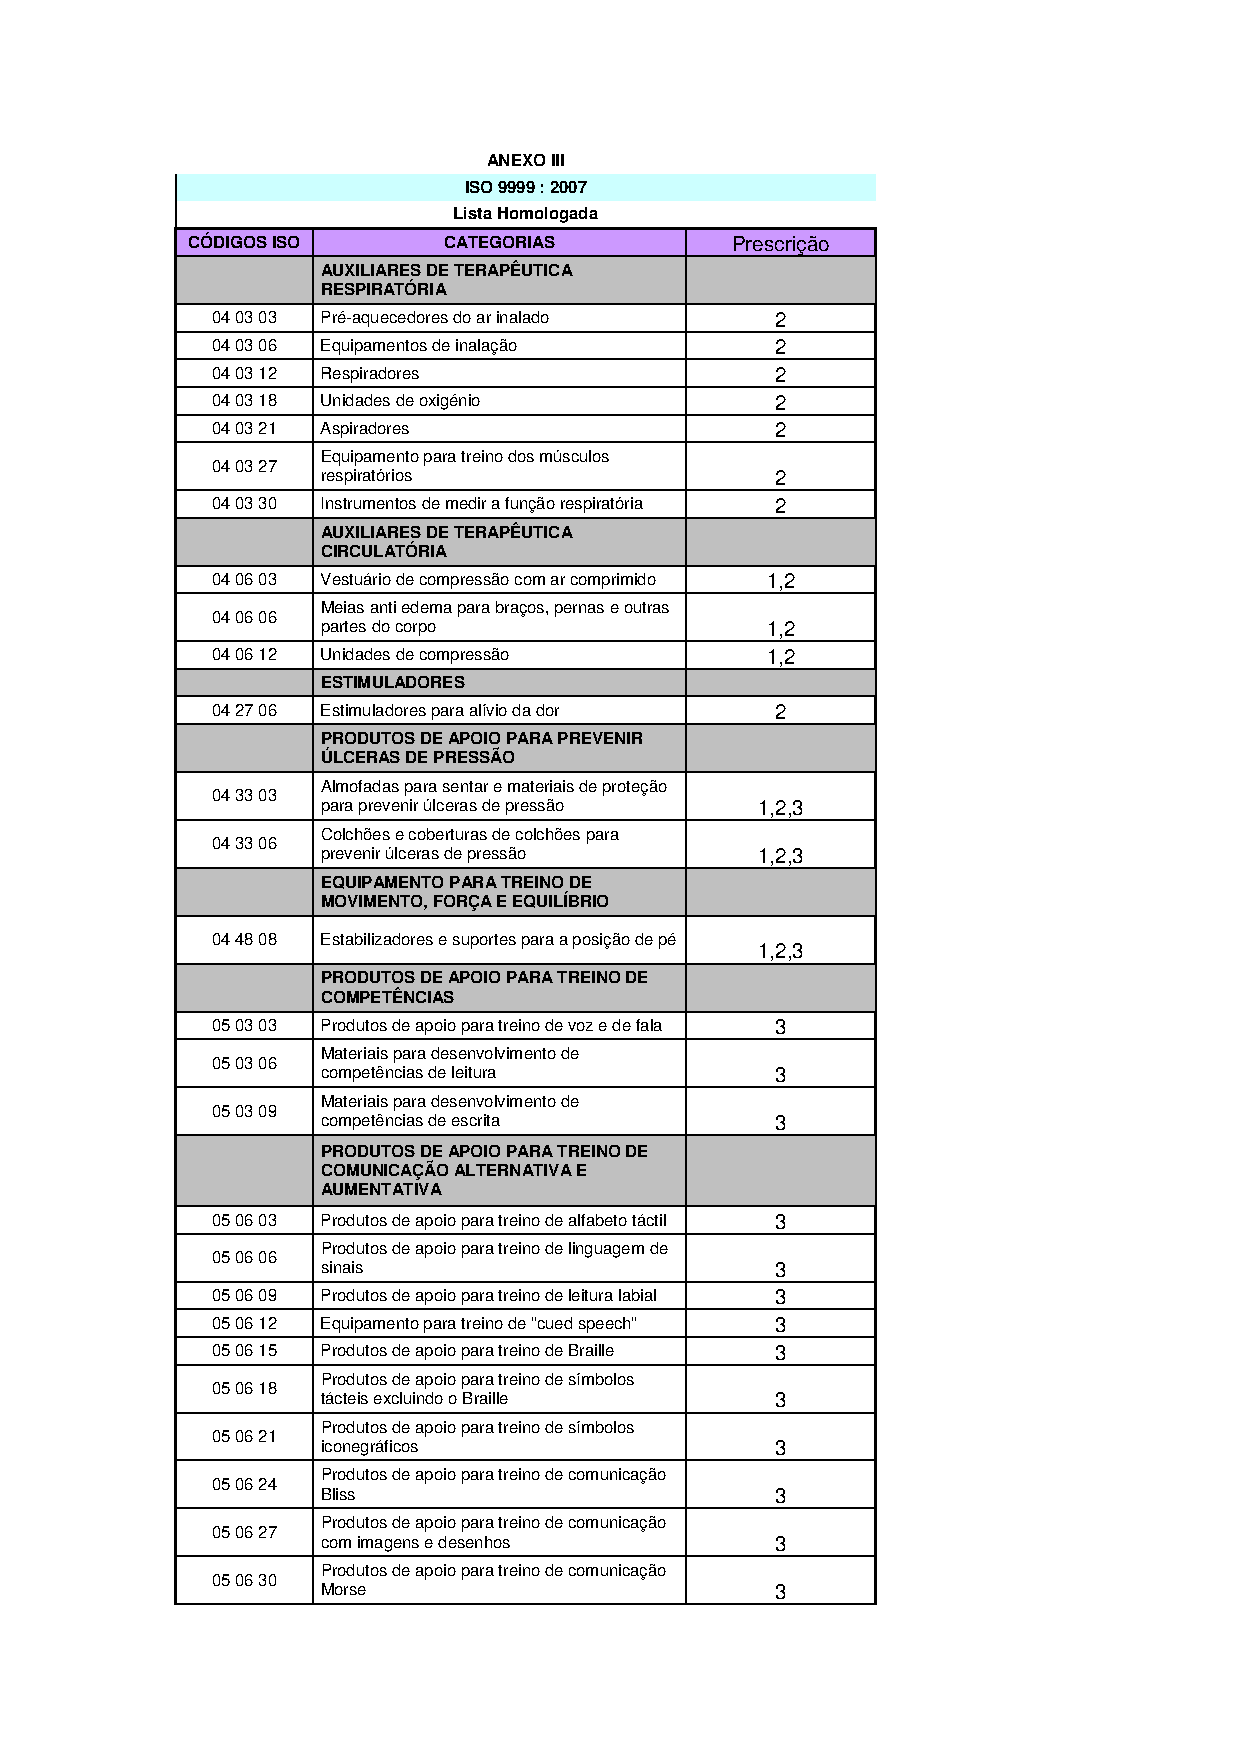
\includegraphics[page=1,scale=0.7]{artigos/iso9999.pdf}\\
    
    \label{fig:arvore}
  \end{center}
\end{figure}
\newpage
\section{Termo de Consentimento Livre e Esclarecido}
\label{apendice2}
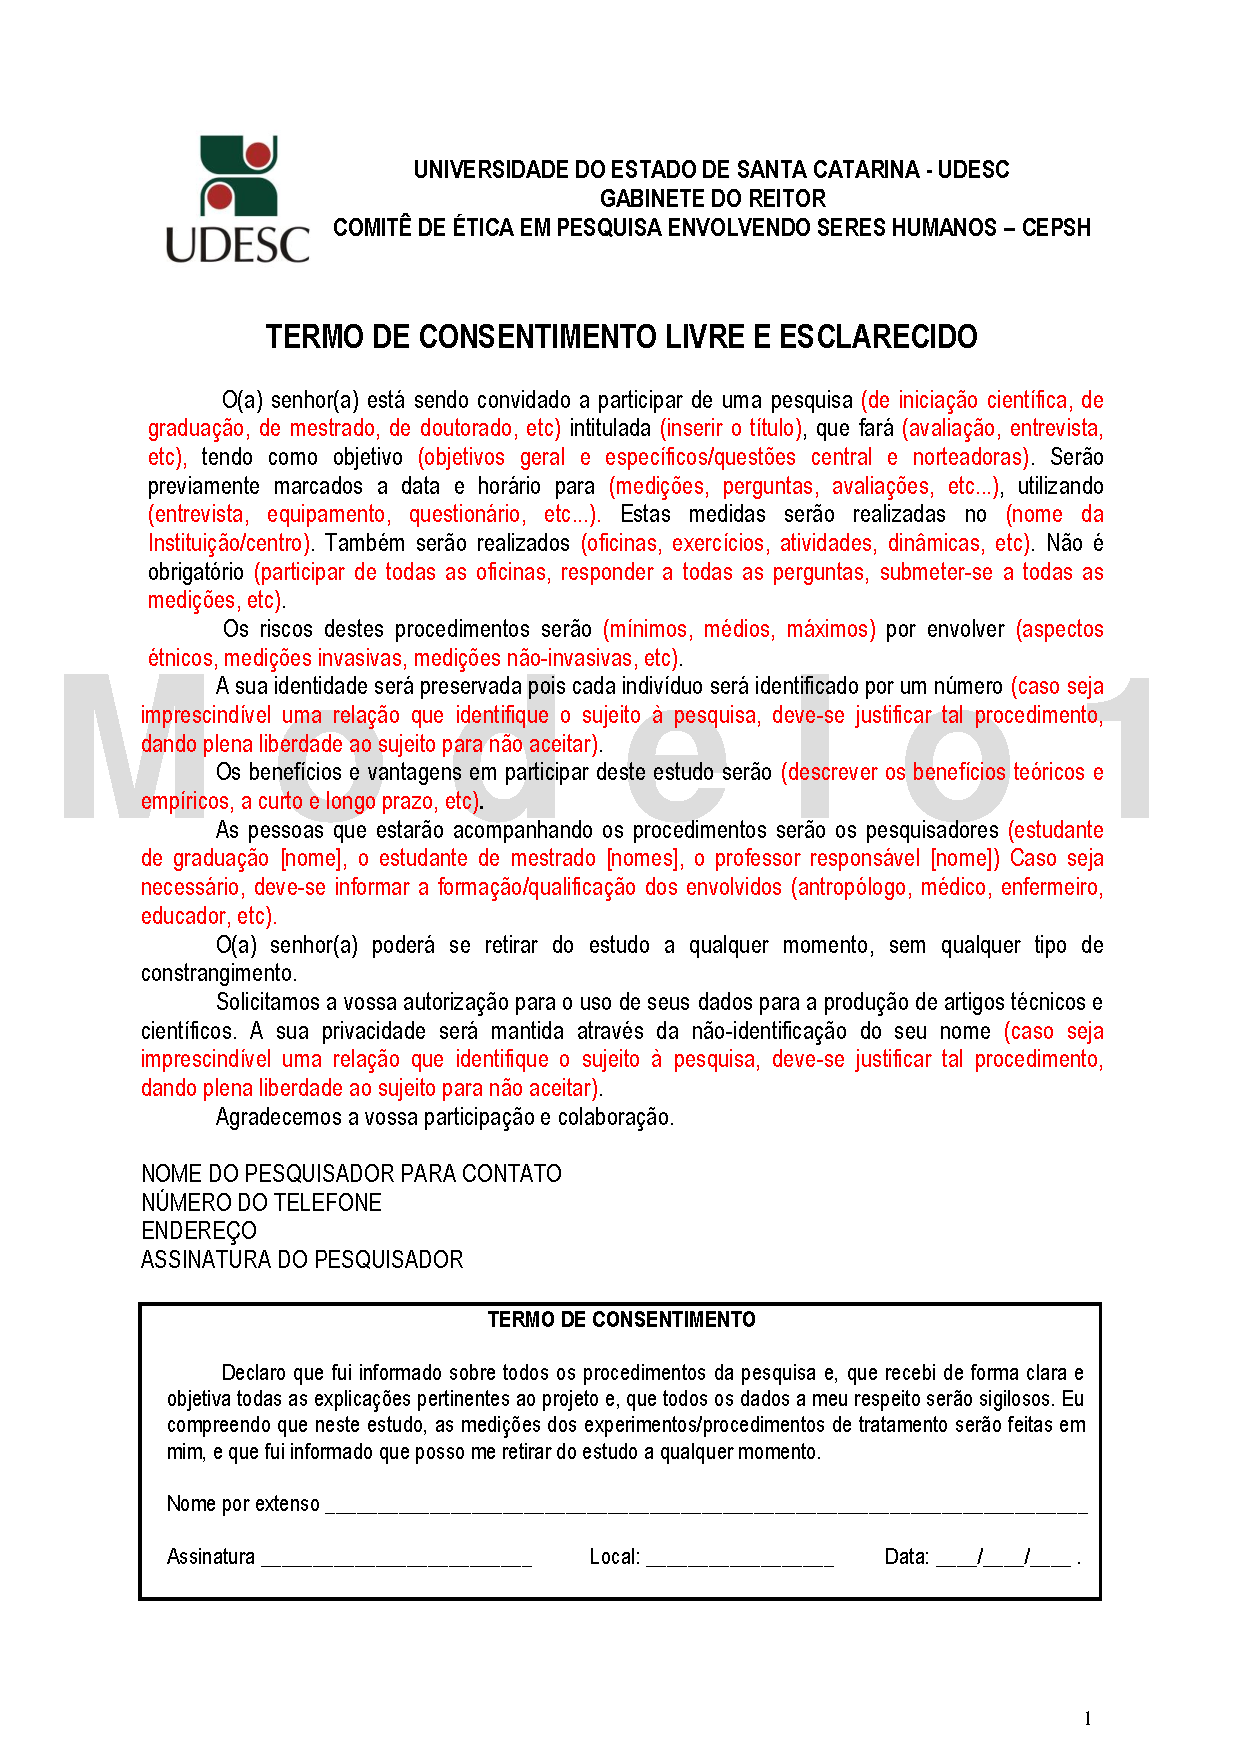
\includegraphics[scale=0.8]{imagens/termo.pdf}
		       %chamada de arquivo anexo.tex
\appendix
\chapter{Ap�ndice}
\renewcommand{\thesection}{\Alph{section}}
\section{Quadros Cl�nicos de Paralisia Cerebral}
\label{apendice1}
\begin{enumerate}
\item {Hemiplegia : � a manifesta��o mais frequente, com
maior comprometimento do membro superior;
acompanha-se de sinais de libera��o tais como
espasticidade , hiper reflexia e sinal de Babinski. O
paciente assume atitude em semiflex�o do membro
superior, permanecendo o membro inferior
hiperestendido e aduzido, e o p� em postura equinovara.
� comum hipotrofia dos segmentos acometidos, sendo
tamb�m poss�vel a ocorr�ncia de outras hemi-hipoestesia
ou hemianopsia.}
\item{ Hemiplegia bilateral ( tetra ou quadriplegia) :
Ocorrem de 9 a 43\% dos pacientes. Ocorrem les�es
difusas bilateral no sistema piramidal dando al�m da
grave tetraparesia esp�stica com intensas retra��es em
semiflex�o, s�ndrome pseudobulbar (hipomimia, disfagia
e disartria), podendo ocorrer ainda microcefalia,
defici�ncia mental e epilepsia.}
\item{Diplegia : Ocorre em 10 a 30 \% dos pacientes, sendo
a forma mais encontrada em prematuros. Tratase de um
comprometimento dos membros inferiores, comumente
evidenciando uma acentuada hipertonia dos adutores,
que configura em alguns doentes o aspecto semiol�gico
denominado s�ndrome de Little (postura com cruzamento
dos membros inferiores e marcha em tesoura). H� 
diferentes grada��es quanto � intensidade do dist�rbio,
podendo ser pouco afetado (tendo recupera��o e bom
progn�stico  adaptam-se � vida di�ria); enquanto outros
evoluem mal com graves limita��es funcionais. Os dados
semiol�gicos s�o muito vari�veis. No 1� ano de vida, a
crian�a apresenta-se hipot�nica, evoluindo
gradativamente para uma outra fase em que se observa
um quadro de distonia intermitente, com tend�ncia ao
opist�tono quando estimulada. Nos casos mais graves a
crian�a pode permanecer num destes est�gios por toda
a sua vida, por�m geralmente passa a exibir hipertonia
esp�stica, inicialmente extensora e, finalmente, com
graves retra��es semiflexoras.}
\item{Discinesia : Atualmente � a mais rara, pois
manifesta-se atrav�s de movimentos involunt�rios,
sobretudo distonias axiais e/ou movimentos c�reoatet�ides
das extremidades. No primeiro ano de vida este
padr�o costuma n�o estar definido, podendo existir
hipotonia muscular. Em geral, quando estes pacientes
est�o relaxados a movimenta��o passiva � facilitada.}
\item{Ataxia : Igualmente rara. Inicialmente pode traduzir se
por hipotonia e, aos poucos, verificam-se altera��es
do equil�brio (ataxia axial) e, menos comumente, da
coordena��o ( ataxia apendicular). Sua marcha se faz com
aumento da base de sustenta��o podendo apresentar
tremor intencional.}
\item{Formas mistas : � a associa��o das manifesta��es
anteriores, correspondendo, geralmente, ao encontro de
movimentos dist�nicos e c�reo atet�ides ou �
combina��o de ataxia com plegia (sobretudo diplegia).
No total, cerca de 75\% dos pacientes doentes com
paralisia cerebral apresentam padr�o esp�stico.
Al�m do dist�rbio motor, obrigat�rio para a
caracteriza��o da paralisia cerebral, o quadro cl�nico pode
incluir tamb�m outras manifesta��es acess�rias com
frequ�ncia vari�vel: 
\begin{enumerate}
\item{ Defici�ncia mental: Ocorre de 30 a
70\% dos pacientes. Est� mais associada �s formas
tetrapl�gicas, dipl�gicas ou mistas;}
\item{ Epilepsia: Varia de
25 a 35\% dos casos, ocorrendo mais associado com a
forma hemipl�gica ou tetrapl�gica; }
\item{ Dist�rbios da
linguagem; }
\item{ Dist�rbios visuais : Pode ocorrer perda da
acuidade visual ou dos movimentos oculares
\(estrabismo\); }
\item{ Dist�rbios do comportamento : S�o mais
comuns nas crian�as com intelig�ncia normal ou lim�trofe,
que se sentem frustradas pela sua limita��o motora,
quadro agravado em alguns casos pela super prote��o
ou rejei��o familiar; e}
\item{ Dist�rbios ortop�dicos : Mesmo
nos pacientes submetidos � reabilita��o bem orientada,
s�o comuns retra��es fibrotend�neas \(50\%\) cifoescoliose
\(15\%\), coxa valga \(5\%\) e deformidades nos p�s.
Todos esses dist�rbios se d�o devido a altera��es
nas �reas motoras cerebrais espec�ficas durante a
inf�ncia.}
\end{enumerate}
}
\end{enumerate}
\newpage
\section{Entrevista}
\label{entrevista}
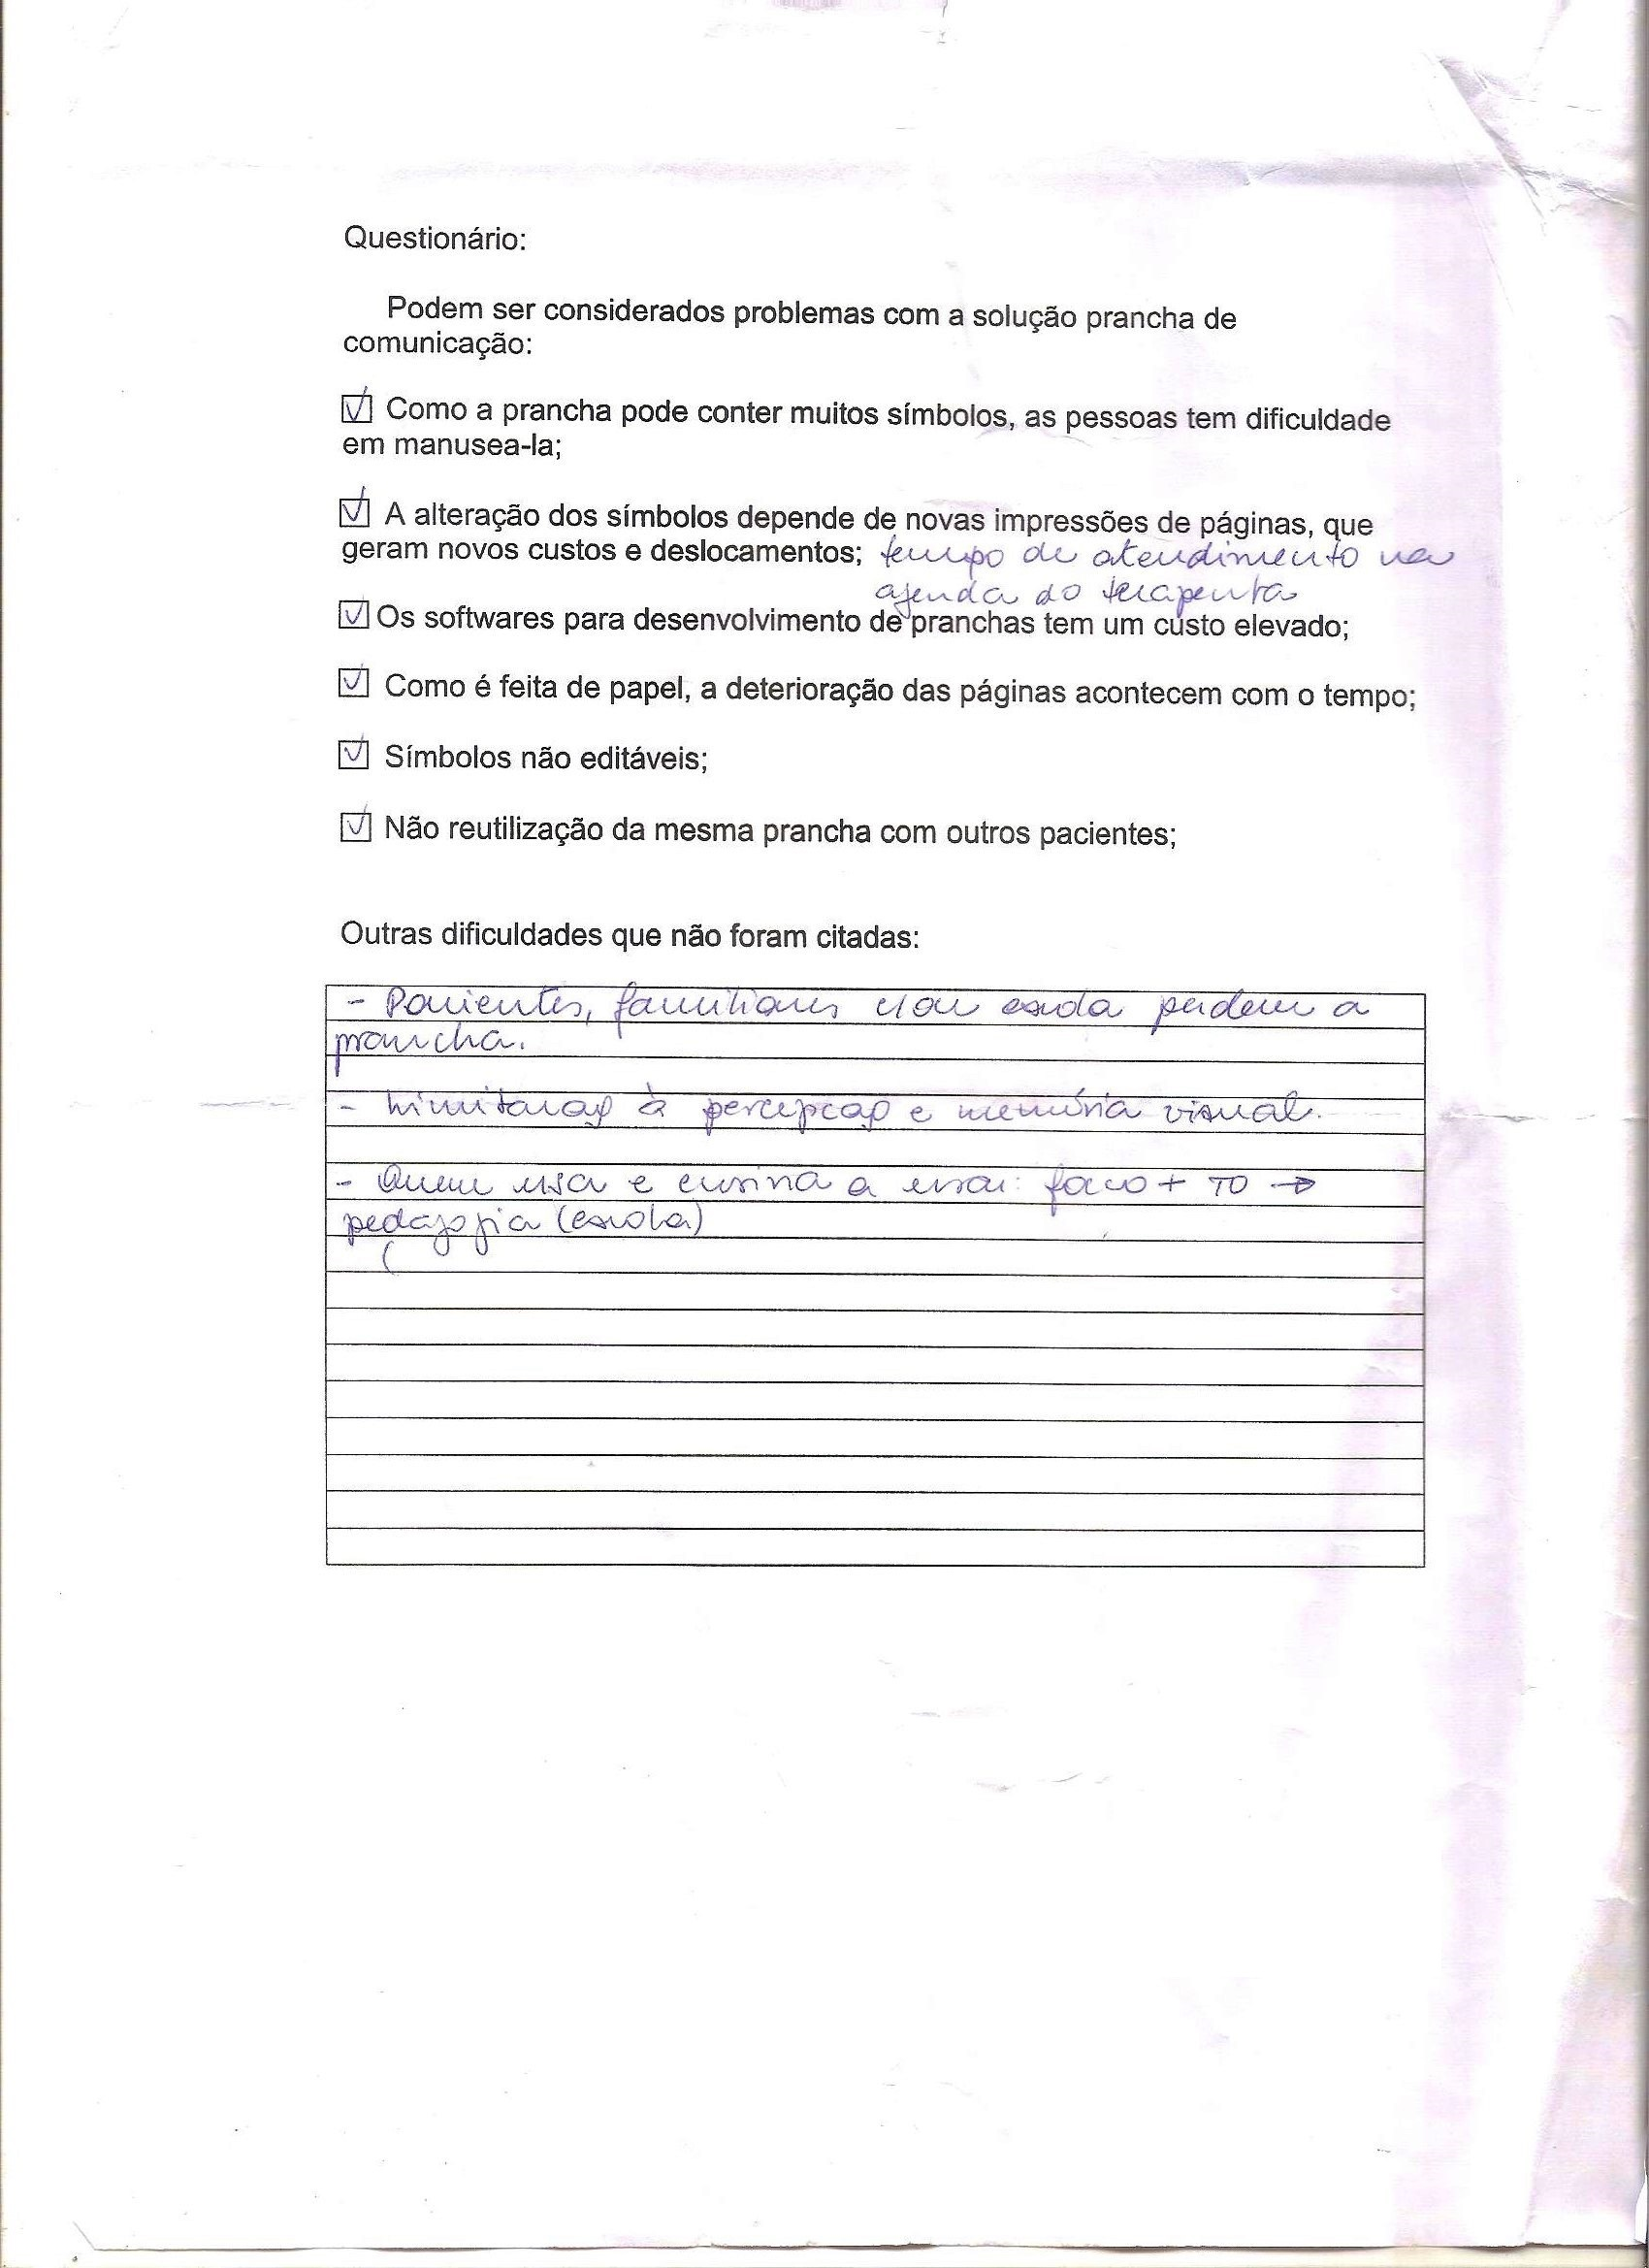
\includegraphics[scale=0.8]{imagens/entrevista.jpg}
	               %chamada de arquivo apendice.tex
\end{document}